\documentclass[1p]{elsarticle_modified}
%\bibliographystyle{elsarticle-num}

%\usepackage[colorlinks]{hyperref}
%\usepackage{abbrmath_seonhwa} %\Abb, \Ascr, \Acal ,\Abf, \Afrak
\usepackage{amsfonts}
\usepackage{amssymb}
\usepackage{amsmath}
\usepackage{amsthm}
\usepackage{scalefnt}
\usepackage{amsbsy}
\usepackage{kotex}
\usepackage{caption}
\usepackage{subfig}
\usepackage{color}
\usepackage{graphicx}
\usepackage{xcolor} %% white, black, red, green, blue, cyan, magenta, yellow
\usepackage{float}
\usepackage{setspace}
\usepackage{hyperref}

\usepackage{tikz}
\usetikzlibrary{arrows}

\usepackage{multirow}
\usepackage{array} % fixed length table
\usepackage{hhline}

%%%%%%%%%%%%%%%%%%%%%
\makeatletter
\renewcommand*\env@matrix[1][\arraystretch]{%
	\edef\arraystretch{#1}%
	\hskip -\arraycolsep
	\let\@ifnextchar\new@ifnextchar
	\array{*\c@MaxMatrixCols c}}
\makeatother %https://tex.stackexchange.com/questions/14071/how-can-i-increase-the-line-spacing-in-a-matrix
%%%%%%%%%%%%%%%

\usepackage[normalem]{ulem}

\newcommand{\msout}[1]{\ifmmode\text{\sout{\ensuremath{#1}}}\else\sout{#1}\fi}
%SOURCE: \msout is \stkout macro in https://tex.stackexchange.com/questions/20609/strikeout-in-math-mode

\newcommand{\cancel}[1]{
	\ifmmode
	{\color{red}\msout{#1}}
	\else
	{\color{red}\sout{#1}}
	\fi
}

\newcommand{\add}[1]{
	{\color{blue}\uwave{#1}}
}

\newcommand{\replace}[2]{
	\ifmmode
	{\color{red}\msout{#1}}{\color{blue}\uwave{#2}}
	\else
	{\color{red}\sout{#1}}{\color{blue}\uwave{#2}}
	\fi
}

\newcommand{\Sol}{\mathcal{S}} %segment
\newcommand{\D}{D} %diagram
\newcommand{\A}{\mathcal{A}} %arc


%%%%%%%%%%%%%%%%%%%%%%%%%%%%%5 test

\def\sl{\operatorname{\textup{SL}}(2,\Cbb)}
\def\psl{\operatorname{\textup{PSL}}(2,\Cbb)}
\def\quan{\mkern 1mu \triangleright \mkern 1mu}

\theoremstyle{definition}
\newtheorem{thm}{Theorem}[section]
\newtheorem{prop}[thm]{Proposition}
\newtheorem{lem}[thm]{Lemma}
\newtheorem{ques}[thm]{Question}
\newtheorem{cor}[thm]{Corollary}
\newtheorem{defn}[thm]{Definition}
\newtheorem{exam}[thm]{Example}
\newtheorem{rmk}[thm]{Remark}
\newtheorem{alg}[thm]{Algorithm}

\newcommand{\I}{\sqrt{-1}}
\begin{document}

%\begin{frontmatter}
%
%\title{Boundary parabolic representations of knots up to 8 crossings}
%
%%% Group authors per affiliation:
%\author{Yunhi Cho} 
%\address{Department of Mathematics, University of Seoul, Seoul, Korea}
%\ead{yhcho@uos.ac.kr}
%
%
%\author{Seonhwa Kim} %\fnref{s_kim}}
%\address{Center for Geometry and Physics, Institute for Basic Science, Pohang, 37673, Korea}
%\ead{ryeona17@ibs.re.kr}
%
%\author{Hyuk Kim}
%\address{Department of Mathematical Sciences, Seoul National University, Seoul 08826, Korea}
%\ead{hyukkim@snu.ac.kr}
%
%\author{Seokbeom Yoon}
%\address{Department of Mathematical Sciences, Seoul National University, Seoul, 08826,  Korea}
%\ead{sbyoon15@snu.ac.kr}
%
%\begin{abstract}
%We find all boundary parabolic representation of knots up to 8 crossings.
%
%\end{abstract}
%\begin{keyword}
%    \MSC[2010] 57M25 
%\end{keyword}
%
%\end{frontmatter}

%\linenumbers
%\tableofcontents
%
\newcommand\colored[1]{\textcolor{white}{\rule[-0.35ex]{0.8em}{1.4ex}}\kern-0.8em\color{red} #1}%
%\newcommand\colored[1]{\textcolor{white}{ #1}\kern-2.17ex	\textcolor{white}{ #1}\kern-1.81ex	\textcolor{white}{ #1}\kern-2.15ex\color{red}#1	}

{\Large $\underline{12a_{1021}~(K12a_{1021})}$}

\setlength{\tabcolsep}{10pt}
\renewcommand{\arraystretch}{1.6}
\vspace{1cm}\begin{tabular}{m{100pt}>{\centering\arraybackslash}m{274pt}}
\multirow{5}{120pt}{
	\centering
	\includegraphics[width=112pt]{../../../GIT/diagram.site/Diagrams/png/1822_12a_1021.png}\\
\ \ \ A knot diagram\footnotemark}&
\allowdisplaybreaks
\textbf{Linearized knot diagam} \\
\cline{2-2}
 &
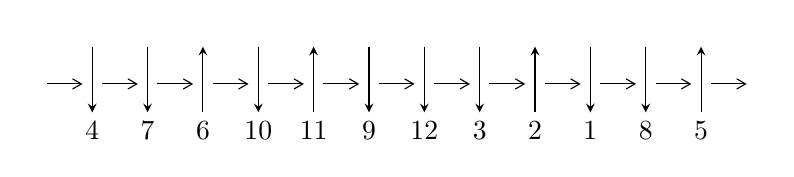
\begin{tikzpicture}[x=20pt, y=17pt]
	% nodes
	\node (C0) at (0, 0) {};
	\node (C1) at (1, 0) {};
	\node (C1U) at (1, +1) {};
	\node (C1D) at (1, -1) {4};

	\node (C2) at (2, 0) {};
	\node (C2U) at (2, +1) {};
	\node (C2D) at (2, -1) {7};

	\node (C3) at (3, 0) {};
	\node (C3U) at (3, +1) {};
	\node (C3D) at (3, -1) {6};

	\node (C4) at (4, 0) {};
	\node (C4U) at (4, +1) {};
	\node (C4D) at (4, -1) {10};

	\node (C5) at (5, 0) {};
	\node (C5U) at (5, +1) {};
	\node (C5D) at (5, -1) {11};

	\node (C6) at (6, 0) {};
	\node (C6U) at (6, +1) {};
	\node (C6D) at (6, -1) {9};

	\node (C7) at (7, 0) {};
	\node (C7U) at (7, +1) {};
	\node (C7D) at (7, -1) {12};

	\node (C8) at (8, 0) {};
	\node (C8U) at (8, +1) {};
	\node (C8D) at (8, -1) {3};

	\node (C9) at (9, 0) {};
	\node (C9U) at (9, +1) {};
	\node (C9D) at (9, -1) {2};

	\node (C10) at (10, 0) {};
	\node (C10U) at (10, +1) {};
	\node (C10D) at (10, -1) {1};

	\node (C11) at (11, 0) {};
	\node (C11U) at (11, +1) {};
	\node (C11D) at (11, -1) {8};

	\node (C12) at (12, 0) {};
	\node (C12U) at (12, +1) {};
	\node (C12D) at (12, -1) {5};
	\node (C13) at (13, 0) {};

	% arrows
	\draw[->,>={angle 60}]
	(C0) edge (C1) (C1) edge (C2) (C2) edge (C3) (C3) edge (C4) (C4) edge (C5) (C5) edge (C6) (C6) edge (C7) (C7) edge (C8) (C8) edge (C9) (C9) edge (C10) (C10) edge (C11) (C11) edge (C12) (C12) edge (C13) ;	\draw[->,>=stealth]
	(C1U) edge (C1D) (C2U) edge (C2D) (C3D) edge (C3U) (C4U) edge (C4D) (C5D) edge (C5U) (C6U) edge (C6D) (C7U) edge (C7D) (C8U) edge (C8D) (C9D) edge (C9U) (C10U) edge (C10D) (C11U) edge (C11D) (C12D) edge (C12U) ;
	\end{tikzpicture} \\
\hhline{~~} \\& 
\textbf{Solving Sequence} \\ \cline{2-2} 
 &
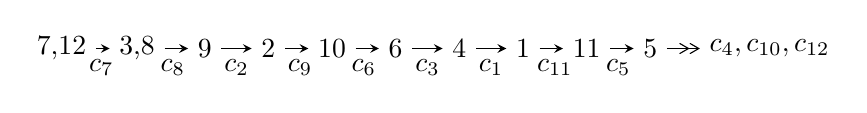
\begin{tikzpicture}[x=23pt, y=7pt]
	% node
	\node (A0) at (-1/8, 0) {7,12};
	\node (A1) at (17/16, 0) {3,8};
	\node (A2) at (17/8, 0) {9};
	\node (A3) at (25/8, 0) {2};
	\node (A4) at (33/8, 0) {10};
	\node (A5) at (41/8, 0) {6};
	\node (A6) at (49/8, 0) {4};
	\node (A7) at (57/8, 0) {1};
	\node (A8) at (65/8, 0) {11};
	\node (A9) at (73/8, 0) {5};
	\node (C1) at (1/2, -1) {$c_{7}$};
	\node (C2) at (13/8, -1) {$c_{8}$};
	\node (C3) at (21/8, -1) {$c_{2}$};
	\node (C4) at (29/8, -1) {$c_{9}$};
	\node (C5) at (37/8, -1) {$c_{6}$};
	\node (C6) at (45/8, -1) {$c_{3}$};
	\node (C7) at (53/8, -1) {$c_{1}$};
	\node (C8) at (61/8, -1) {$c_{11}$};
	\node (C9) at (69/8, -1) {$c_{5}$};
	\node (A10) at (11, 0) {$c_{4},c_{10},c_{12}$};

	% edge
	\draw[->,>=stealth]	
	(A0) edge (A1) (A1) edge (A2) (A2) edge (A3) (A3) edge (A4) (A4) edge (A5) (A5) edge (A6) (A6) edge (A7) (A7) edge (A8) (A8) edge (A9) ;
	\draw[->>,>={angle 60}]	
	(A9) edge (A10);
\end{tikzpicture} \\ 

\end{tabular} \\

\footnotetext{
The image of knot diagram is generated by the software ``\textbf{Draw programme}" developed by Andrew Bartholomew(\url{http://www.layer8.co.uk/maths/draw/index.htm\#Running-draw}), where we modified some parts for our purpose(\url{https://github.com/CATsTAILs/LinksPainter}).
}\phantom \\ \newline 
\centering \textbf{Ideals for irreducible components\footnotemark of $X_{\text{par}}$} 
 
\begin{align*}
I^u_{1}&=\langle 
3.76415\times10^{1746} u^{228}+7.91396\times10^{1745} u^{227}+\cdots+8.71926\times10^{1748} b-1.55984\times10^{1750},\\
\phantom{I^u_{1}}&\phantom{= \langle  }-4.25186\times10^{1751} u^{228}+3.67618\times10^{1751} u^{227}+\cdots+1.12853\times10^{1753} a-1.14813\times10^{1755},\\
\phantom{I^u_{1}}&\phantom{= \langle  }u^{229}- u^{228}+\cdots-473 u-1849\rangle \\
I^u_{2}&=\langle 
-2.54531\times10^{91} u^{59}-2.65678\times10^{92} u^{58}+\cdots+1.32675\times10^{91} b+1.11176\times10^{93},\\
\phantom{I^u_{2}}&\phantom{= \langle  }6.49994\times10^{93} u^{59}+1.67375\times10^{94} u^{58}+\cdots+9.28722\times10^{91} a-1.04402\times10^{94},\;u^{60}+2 u^{59}+\cdots-2 u-1\rangle \\
\\
\end{align*}
\raggedright * 2 irreducible components of $\dim_{\mathbb{C}}=0$, with total 289 representations.\\
\footnotetext{All coefficients of polynomials are rational numbers. But the coefficients are sometimes approximated in decimal forms when there is not enough margin.}
\newpage
\renewcommand{\arraystretch}{1}
\centering \section*{I. $I^u_{1}= \langle 3.76\times10^{1746} u^{228}+7.91\times10^{1745} u^{227}+\cdots+8.72\times10^{1748} b-1.56\times10^{1750},\;-4.25\times10^{1751} u^{228}+3.68\times10^{1751} u^{227}+\cdots+1.13\times10^{1753} a-1.15\times10^{1755},\;u^{229}- u^{228}+\cdots-473 u-1849 \rangle$}
\flushleft \textbf{(i) Arc colorings}\\
\begin{tabular}{m{7pt} m{180pt} m{7pt} m{180pt} }
\flushright $a_{7}=$&$\begin{pmatrix}1\\0\end{pmatrix}$ \\
\flushright $a_{12}=$&$\begin{pmatrix}0\\u\end{pmatrix}$ \\
\flushright $a_{3}=$&$\begin{pmatrix}0.0376759 u^{228}-0.0325749 u^{227}+\cdots-88.3676 u+101.736\\-0.00431706 u^{228}-0.000907642 u^{227}+\cdots+79.3362 u+17.8896\end{pmatrix}$ \\
\flushright $a_{8}=$&$\begin{pmatrix}1\\u^2\end{pmatrix}$ \\
\flushright $a_{9}=$&$\begin{pmatrix}0.0111369 u^{228}-0.00773449 u^{227}+\cdots+1.61264 u+31.0373\\-0.000822677 u^{228}-0.000737425 u^{227}+\cdots+38.2191 u+12.9938\end{pmatrix}$ \\
\flushright $a_{2}=$&$\begin{pmatrix}0.0333589 u^{228}-0.0334825 u^{227}+\cdots-9.03142 u+119.626\\-0.00431706 u^{228}-0.000907642 u^{227}+\cdots+79.3362 u+17.8896\end{pmatrix}$ \\
\flushright $a_{10}=$&$\begin{pmatrix}0.0120323 u^{228}-0.00969198 u^{227}+\cdots+20.8382 u+29.8733\\-0.000112845 u^{228}-0.00116653 u^{227}+\cdots+17.8629 u+3.86081\end{pmatrix}$ \\
\flushright $a_{6}=$&$\begin{pmatrix}-0.000233471 u^{228}-0.00328437 u^{227}+\cdots+17.8662 u+9.63263\\-0.000608332 u^{228}-0.000133445 u^{227}+\cdots+6.30555 u+2.83195\end{pmatrix}$ \\
\flushright $a_{4}=$&$\begin{pmatrix}0.0130573 u^{228}-0.0170195 u^{227}+\cdots-17.4157 u+46.6706\\-0.00640952 u^{228}+0.00156866 u^{227}+\cdots+59.5530 u+7.53289\end{pmatrix}$ \\
\flushright $a_{1}=$&$\begin{pmatrix}0.00882879 u^{228}-0.00585265 u^{227}+\cdots+8.93288 u+11.2640\\0.00101762 u^{228}-0.00257083 u^{227}+\cdots+10.1225 u+8.25939\end{pmatrix}$ \\
\flushright $a_{11}=$&$\begin{pmatrix}u\\u^3+u\end{pmatrix}$ \\
\flushright $a_{5}=$&$\begin{pmatrix}-0.00189729 u^{228}-0.00136916 u^{227}+\cdots+12.3347 u+4.76550\\-0.00128529 u^{228}+0.00117240 u^{227}+\cdots-2.18353 u-1.57035\end{pmatrix}$\\&\end{tabular}
\flushleft \textbf{(ii) Obstruction class $= -1$}\\~\\
\flushleft \textbf{(iii) Cusp Shapes $= 0.0187149 u^{228}-0.0269520 u^{227}+\cdots+500.292 u+157.998$}\\~\\
\newpage\renewcommand{\arraystretch}{1}
\flushleft \textbf{(iv) u-Polynomials at the component}\newline \\
\begin{tabular}{m{50pt}|m{274pt}}
Crossings & \hspace{64pt}u-Polynomials at each crossing \\
\hline $$\begin{aligned}c_{1}\end{aligned}$$&$\begin{aligned}
&u^{229}+13 u^{228}+\cdots-211 u+4
\end{aligned}$\\
\hline $$\begin{aligned}c_{2}\end{aligned}$$&$\begin{aligned}
&u^{229}+u^{228}+\cdots+22552586 u-1584023
\end{aligned}$\\
\hline $$\begin{aligned}c_{3}\end{aligned}$$&$\begin{aligned}
&u^{229}-9 u^{228}+\cdots-2711301018 u-134641844
\end{aligned}$\\
\hline $$\begin{aligned}c_{4}\end{aligned}$$&$\begin{aligned}
&7(7 u^{229}-72 u^{228}+\cdots-235032 u+85717)
\end{aligned}$\\
\hline $$\begin{aligned}c_{5}\end{aligned}$$&$\begin{aligned}
&7(7 u^{229}-79 u^{228}+\cdots+1.39432\times10^{9} u+5.30079\times10^{7})
\end{aligned}$\\
\hline $$\begin{aligned}c_{6}\end{aligned}$$&$\begin{aligned}
&u^{229}-16 u^{228}+\cdots-127 u+14
\end{aligned}$\\
\hline $$\begin{aligned}c_{7},c_{11}\end{aligned}$$&$\begin{aligned}
&u^{229}- u^{228}+\cdots-473 u-1849
\end{aligned}$\\
\hline $$\begin{aligned}c_{8}\end{aligned}$$&$\begin{aligned}
&7(7 u^{229}-34 u^{228}+\cdots+4 u-1)
\end{aligned}$\\
\hline $$\begin{aligned}c_{9}\end{aligned}$$&$\begin{aligned}
&7(7 u^{229}-69 u^{228}+\cdots-3.58247\times10^{13} u-6.39172\times10^{12})
\end{aligned}$\\
\hline $$\begin{aligned}c_{10}\end{aligned}$$&$\begin{aligned}
&u^{229}-13 u^{228}+\cdots+14718 u-497
\end{aligned}$\\
\hline $$\begin{aligned}c_{12}\end{aligned}$$&$\begin{aligned}
&u^{229}+4 u^{227}+\cdots+603279267 u+17477887
\end{aligned}$\\
\hline
\end{tabular}\\~\\
\newpage\renewcommand{\arraystretch}{1}
\flushleft \textbf{(v) Riley Polynomials at the component}\newline \\
\begin{tabular}{m{50pt}|m{274pt}}
Crossings & \hspace{64pt}Riley Polynomials at each crossing \\
\hline $$\begin{aligned}c_{1}\end{aligned}$$&$\begin{aligned}
&y^{229}-25 y^{228}+\cdots-1479 y-16
\end{aligned}$\\
\hline $$\begin{aligned}c_{2}\end{aligned}$$&$\begin{aligned}
&y^{229}-57 y^{228}+\cdots+343601616258474 y-2509128864529
\end{aligned}$\\
\hline $$\begin{aligned}c_{3}\end{aligned}$$&$\begin{aligned}
&y^{229}+11 y^{228}+\cdots+2.46\times10^{19} y-1.81\times10^{16}
\end{aligned}$\\
\hline $$\begin{aligned}c_{4}\end{aligned}$$&$\begin{aligned}
&49(49 y^{229}-1978 y^{228}+\cdots+8.37639\times10^{11} y-7.34740\times10^{9})
\end{aligned}$\\
\hline $$\begin{aligned}c_{5}\end{aligned}$$&$\begin{aligned}
&49(49 y^{229}-1733 y^{228}+\cdots+1.47012\times10^{18} y-2.80983\times10^{15})
\end{aligned}$\\
\hline $$\begin{aligned}c_{6}\end{aligned}$$&$\begin{aligned}
&y^{229}-30 y^{228}+\cdots-50315 y-196
\end{aligned}$\\
\hline $$\begin{aligned}c_{7},c_{11}\end{aligned}$$&$\begin{aligned}
&y^{229}+105 y^{228}+\cdots-189798001 y-3418801
\end{aligned}$\\
\hline $$\begin{aligned}c_{8}\end{aligned}$$&$\begin{aligned}
&49(49 y^{229}+734 y^{228}+\cdots+264 y-1)
\end{aligned}$\\
\hline $$\begin{aligned}c_{9}\end{aligned}$$&$\begin{aligned}
&49(49 y^{229}+6369 y^{228}+\cdots+3.98090\times10^{27} y-4.08541\times10^{25})
\end{aligned}$\\
\hline $$\begin{aligned}c_{10}\end{aligned}$$&$\begin{aligned}
&y^{229}+11 y^{228}+\cdots+96513510 y-247009
\end{aligned}$\\
\hline $$\begin{aligned}c_{12}\end{aligned}$$&$\begin{aligned}
&y^{229}+8 y^{228}+\cdots-17329253455415529 y-305476533984769
\end{aligned}$\\
\hline
\end{tabular}\\~\\
\newpage\flushleft \textbf{(vi) Complex Volumes and Cusp Shapes}
$$\begin{array}{c|c|c}  
\text{Solutions to }I^u_{1}& \I (\text{vol} + \sqrt{-1}CS) & \text{Cusp shape}\\
 \hline 
\begin{aligned}
u &= \phantom{-}0.906958 + 0.409673 I \\
a &= \phantom{-}0.116480 + 0.115295 I \\
b &= \phantom{-}1.066970 - 0.758273 I\end{aligned}
 & -1.44153 + 7.88127 I & \phantom{-0.000000 } 0 \\ \hline\begin{aligned}
u &= \phantom{-}0.906958 - 0.409673 I \\
a &= \phantom{-}0.116480 - 0.115295 I \\
b &= \phantom{-}1.066970 + 0.758273 I\end{aligned}
 & -1.44153 - 7.88127 I & \phantom{-0.000000 } 0 \\ \hline\begin{aligned}
u &= -0.474703 + 0.889311 I \\
a &= -1.65106 + 0.72293 I \\
b &= -0.610238 - 0.110691 I\end{aligned}
 & \phantom{-}0.18145 + 3.52728 I & \phantom{-0.000000 } 0 \\ \hline\begin{aligned}
u &= -0.474703 - 0.889311 I \\
a &= -1.65106 - 0.72293 I \\
b &= -0.610238 + 0.110691 I\end{aligned}
 & \phantom{-}0.18145 - 3.52728 I & \phantom{-0.000000 } 0 \\ \hline\begin{aligned}
u &= \phantom{-}0.264499 + 0.974265 I \\
a &= \phantom{-}0.03961 + 1.82145 I \\
b &= -0.259492 - 0.091492 I\end{aligned}
 & -0.36760 + 2.12715 I & \phantom{-0.000000 } 0 \\ \hline\begin{aligned}
u &= \phantom{-}0.264499 - 0.974265 I \\
a &= \phantom{-}0.03961 - 1.82145 I \\
b &= -0.259492 + 0.091492 I\end{aligned}
 & -0.36760 - 2.12715 I & \phantom{-0.000000 } 0 \\ \hline\begin{aligned}
u &= -0.502388 + 0.879806 I \\
a &= \phantom{-}4.58739 + 2.40439 I \\
b &= \phantom{-}0.194447 - 0.110337 I\end{aligned}
 & -0.00477725 - 0.01159600 I & \phantom{-0.000000 } 0 \\ \hline\begin{aligned}
u &= -0.502388 - 0.879806 I \\
a &= \phantom{-}4.58739 - 2.40439 I \\
b &= \phantom{-}0.194447 + 0.110337 I\end{aligned}
 & -0.00477725 + 0.01159600 I & \phantom{-0.000000 } 0 \\ \hline\begin{aligned}
u &= \phantom{-}0.271744 + 0.941972 I \\
a &= \phantom{-}0.972223 + 0.468581 I \\
b &= -1.98624 + 0.01846 I\end{aligned}
 & -0.93497 - 6.19073 I & \phantom{-0.000000 } 0 \\ \hline\begin{aligned}
u &= \phantom{-}0.271744 - 0.941972 I \\
a &= \phantom{-}0.972223 - 0.468581 I \\
b &= -1.98624 - 0.01846 I\end{aligned}
 & -0.93497 + 6.19073 I & \phantom{-0.000000 } 0\\
 \hline 
 \end{array}$$\newpage$$\begin{array}{c|c|c}  
\text{Solutions to }I^u_{1}& \I (\text{vol} + \sqrt{-1}CS) & \text{Cusp shape}\\
 \hline 
\begin{aligned}
u &= \phantom{-}0.425560 + 0.881710 I \\
a &= \phantom{-}0.25405 - 2.12175 I \\
b &= \phantom{-}1.61719 + 0.26169 I\end{aligned}
 & \phantom{-}4.68790 - 1.75468 I & \phantom{-0.000000 } 0 \\ \hline\begin{aligned}
u &= \phantom{-}0.425560 - 0.881710 I \\
a &= \phantom{-}0.25405 + 2.12175 I \\
b &= \phantom{-}1.61719 - 0.26169 I\end{aligned}
 & \phantom{-}4.68790 + 1.75468 I & \phantom{-0.000000 } 0 \\ \hline\begin{aligned}
u &= \phantom{-}0.276047 + 0.938953 I \\
a &= -1.264410 + 0.427067 I \\
b &= -0.917140 - 0.209970 I\end{aligned}
 & -0.36391 - 4.29694 I & \phantom{-0.000000 } 0 \\ \hline\begin{aligned}
u &= \phantom{-}0.276047 - 0.938953 I \\
a &= -1.264410 - 0.427067 I \\
b &= -0.917140 + 0.209970 I\end{aligned}
 & -0.36391 + 4.29694 I & \phantom{-0.000000 } 0 \\ \hline\begin{aligned}
u &= -0.822025 + 0.608325 I \\
a &= \phantom{-}0.376375 - 0.023401 I \\
b &= \phantom{-}0.896681 - 0.370881 I\end{aligned}
 & -3.09357 + 4.19138 I & \phantom{-0.000000 } 0 \\ \hline\begin{aligned}
u &= -0.822025 - 0.608325 I \\
a &= \phantom{-}0.376375 + 0.023401 I \\
b &= \phantom{-}0.896681 + 0.370881 I\end{aligned}
 & -3.09357 - 4.19138 I & \phantom{-0.000000 } 0 \\ \hline\begin{aligned}
u &= -0.332020 + 0.912989 I \\
a &= \phantom{-}0.244543 - 1.248450 I \\
b &= \phantom{-}0.720856 + 0.831454 I\end{aligned}
 & \phantom{-}1.39437 + 0.84425 I & \phantom{-0.000000 } 0 \\ \hline\begin{aligned}
u &= -0.332020 - 0.912989 I \\
a &= \phantom{-}0.244543 + 1.248450 I \\
b &= \phantom{-}0.720856 - 0.831454 I\end{aligned}
 & \phantom{-}1.39437 - 0.84425 I & \phantom{-0.000000 } 0 \\ \hline\begin{aligned}
u &= -0.312832 + 0.919047 I \\
a &= -0.26654 + 2.16797 I \\
b &= \phantom{-}1.63479 - 0.33518 I\end{aligned}
 & \phantom{-}4.67033 + 1.30064 I & \phantom{-0.000000 } 0 \\ \hline\begin{aligned}
u &= -0.312832 - 0.919047 I \\
a &= -0.26654 - 2.16797 I \\
b &= \phantom{-}1.63479 + 0.33518 I\end{aligned}
 & \phantom{-}4.67033 - 1.30064 I & \phantom{-0.000000 } 0\\
 \hline 
 \end{array}$$\newpage$$\begin{array}{c|c|c}  
\text{Solutions to }I^u_{1}& \I (\text{vol} + \sqrt{-1}CS) & \text{Cusp shape}\\
 \hline 
\begin{aligned}
u &= -0.539252 + 0.804148 I \\
a &= -0.168601 + 1.042970 I \\
b &= -0.650438 - 0.441958 I\end{aligned}
 & -0.011311 + 0.518705 I & \phantom{-0.000000 } 0 \\ \hline\begin{aligned}
u &= -0.539252 - 0.804148 I \\
a &= -0.168601 - 1.042970 I \\
b &= -0.650438 + 0.441958 I\end{aligned}
 & -0.011311 - 0.518705 I & \phantom{-0.000000 } 0 \\ \hline\begin{aligned}
u &= \phantom{-}0.830682 + 0.482859 I \\
a &= \phantom{-}0.152105 + 0.135066 I \\
b &= -1.122120 + 0.780990 I\end{aligned}
 & -4.56627 + 2.00715 I & \phantom{-0.000000 } 0 \\ \hline\begin{aligned}
u &= \phantom{-}0.830682 - 0.482859 I \\
a &= \phantom{-}0.152105 - 0.135066 I \\
b &= -1.122120 - 0.780990 I\end{aligned}
 & -4.56627 - 2.00715 I & \phantom{-0.000000 } 0 \\ \hline\begin{aligned}
u &= \phantom{-}0.927295 + 0.240852 I \\
a &= -0.490518 - 0.991046 I \\
b &= \phantom{-}0.281663 - 0.706663 I\end{aligned}
 & -4.41110 - 4.72183 I & \phantom{-0.000000 } 0 \\ \hline\begin{aligned}
u &= \phantom{-}0.927295 - 0.240852 I \\
a &= -0.490518 + 0.991046 I \\
b &= \phantom{-}0.281663 + 0.706663 I\end{aligned}
 & -4.41110 + 4.72183 I & \phantom{-0.000000 } 0 \\ \hline\begin{aligned}
u &= -0.440481 + 0.949602 I \\
a &= \phantom{-}0.638864 - 0.499262 I \\
b &= \phantom{-}0.478186 + 0.204843 I\end{aligned}
 & \phantom{-}0.11110 + 3.61465 I & \phantom{-0.000000 } 0 \\ \hline\begin{aligned}
u &= -0.440481 - 0.949602 I \\
a &= \phantom{-}0.638864 + 0.499262 I \\
b &= \phantom{-}0.478186 - 0.204843 I\end{aligned}
 & \phantom{-}0.11110 - 3.61465 I & \phantom{-0.000000 } 0 \\ \hline\begin{aligned}
u &= \phantom{-}0.683211 + 0.664281 I \\
a &= -0.115211 + 0.449876 I \\
b &= -1.45747 + 0.68398 I\end{aligned}
 & -3.97806 + 3.23056 I & \phantom{-0.000000 } 0 \\ \hline\begin{aligned}
u &= \phantom{-}0.683211 - 0.664281 I \\
a &= -0.115211 - 0.449876 I \\
b &= -1.45747 - 0.68398 I\end{aligned}
 & -3.97806 - 3.23056 I & \phantom{-0.000000 } 0\\
 \hline 
 \end{array}$$\newpage$$\begin{array}{c|c|c}  
\text{Solutions to }I^u_{1}& \I (\text{vol} + \sqrt{-1}CS) & \text{Cusp shape}\\
 \hline 
\begin{aligned}
u &= -0.455778 + 0.836071 I \\
a &= -0.67024 - 2.88161 I \\
b &= -0.286861 + 0.224600 I\end{aligned}
 & -0.019576 + 0.314170 I & \phantom{-0.000000 } 0 \\ \hline\begin{aligned}
u &= -0.455778 - 0.836071 I \\
a &= -0.67024 + 2.88161 I \\
b &= -0.286861 - 0.224600 I\end{aligned}
 & -0.019576 - 0.314170 I & \phantom{-0.000000 } 0 \\ \hline\begin{aligned}
u &= -0.325546 + 0.894225 I \\
a &= -0.16841 + 2.63260 I \\
b &= \phantom{-}0.373360 - 1.077690 I\end{aligned}
 & \phantom{-}1.31358 + 1.93521 I & \phantom{-0.000000 } 0 \\ \hline\begin{aligned}
u &= -0.325546 - 0.894225 I \\
a &= -0.16841 - 2.63260 I \\
b &= \phantom{-}0.373360 + 1.077690 I\end{aligned}
 & \phantom{-}1.31358 - 1.93521 I & \phantom{-0.000000 } 0 \\ \hline\begin{aligned}
u &= -0.248454 + 1.024870 I \\
a &= -1.00564 - 1.28481 I \\
b &= \phantom{-}1.03140 + 1.16936 I\end{aligned}
 & \phantom{-}1.85551 + 5.08408 I & \phantom{-0.000000 } 0 \\ \hline\begin{aligned}
u &= -0.248454 - 1.024870 I \\
a &= -1.00564 + 1.28481 I \\
b &= \phantom{-}1.03140 - 1.16936 I\end{aligned}
 & \phantom{-}1.85551 - 5.08408 I & \phantom{-0.000000 } 0 \\ \hline\begin{aligned}
u &= \phantom{-}0.536647 + 0.913795 I \\
a &= -1.106140 + 0.142528 I \\
b &= \phantom{-}0.809525 - 0.757157 I\end{aligned}
 & \phantom{-}3.73635 - 2.80562 I & \phantom{-0.000000 } 0 \\ \hline\begin{aligned}
u &= \phantom{-}0.536647 - 0.913795 I \\
a &= -1.106140 - 0.142528 I \\
b &= \phantom{-}0.809525 + 0.757157 I\end{aligned}
 & \phantom{-}3.73635 + 2.80562 I & \phantom{-0.000000 } 0 \\ \hline\begin{aligned}
u &= -1.061100 + 0.094815 I \\
a &= \phantom{-}0.345944 - 0.446422 I \\
b &= \phantom{-}0.636598 - 0.519522 I\end{aligned}
 & -3.23032 + 2.65620 I & \phantom{-0.000000 } 0 \\ \hline\begin{aligned}
u &= -1.061100 - 0.094815 I \\
a &= \phantom{-}0.345944 + 0.446422 I \\
b &= \phantom{-}0.636598 + 0.519522 I\end{aligned}
 & -3.23032 - 2.65620 I & \phantom{-0.000000 } 0\\
 \hline 
 \end{array}$$\newpage$$\begin{array}{c|c|c}  
\text{Solutions to }I^u_{1}& \I (\text{vol} + \sqrt{-1}CS) & \text{Cusp shape}\\
 \hline 
\begin{aligned}
u &= \phantom{-}0.508447 + 0.937718 I \\
a &= -1.112310 + 0.527044 I \\
b &= \phantom{-}0.875106 - 0.940988 I\end{aligned}
 & \phantom{-}1.72706 - 6.16112 I & \phantom{-0.000000 } 0 \\ \hline\begin{aligned}
u &= \phantom{-}0.508447 - 0.937718 I \\
a &= -1.112310 - 0.527044 I \\
b &= \phantom{-}0.875106 + 0.940988 I\end{aligned}
 & \phantom{-}1.72706 + 6.16112 I & \phantom{-0.000000 } 0 \\ \hline\begin{aligned}
u &= -0.863275 + 0.300409 I \\
a &= \phantom{-}0.209663 + 0.207516 I \\
b &= -0.576860 + 0.238142 I\end{aligned}
 & -1.76315 + 0.27351 I & \phantom{-0.000000 } 0 \\ \hline\begin{aligned}
u &= -0.863275 - 0.300409 I \\
a &= \phantom{-}0.209663 - 0.207516 I \\
b &= -0.576860 - 0.238142 I\end{aligned}
 & -1.76315 - 0.27351 I & \phantom{-0.000000 } 0 \\ \hline\begin{aligned}
u &= -1.092280 + 0.044489 I \\
a &= \phantom{-}0.0974631 - 0.0573280 I \\
b &= \phantom{-}0.898989 + 0.705326 I\end{aligned}
 & -2.52315 - 7.59480 I & \phantom{-0.000000 } 0 \\ \hline\begin{aligned}
u &= -1.092280 - 0.044489 I \\
a &= \phantom{-}0.0974631 + 0.0573280 I \\
b &= \phantom{-}0.898989 - 0.705326 I\end{aligned}
 & -2.52315 + 7.59480 I & \phantom{-0.000000 } 0 \\ \hline\begin{aligned}
u &= \phantom{-}0.386860 + 1.033150 I \\
a &= \phantom{-}0.03958 - 2.19069 I \\
b &= \phantom{-}0.573063 + 0.673251 I\end{aligned}
 & \phantom{-}3.62214 - 6.57281 I & \phantom{-0.000000 } 0 \\ \hline\begin{aligned}
u &= \phantom{-}0.386860 - 1.033150 I \\
a &= \phantom{-}0.03958 + 2.19069 I \\
b &= \phantom{-}0.573063 - 0.673251 I\end{aligned}
 & \phantom{-}3.62214 + 6.57281 I & \phantom{-0.000000 } 0 \\ \hline\begin{aligned}
u &= \phantom{-}0.502491 + 0.994278 I \\
a &= -0.55113 + 2.15848 I \\
b &= -1.27318 - 1.71367 I\end{aligned}
 & -1.91900 - 6.09371 I & \phantom{-0.000000 } 0 \\ \hline\begin{aligned}
u &= \phantom{-}0.502491 - 0.994278 I \\
a &= -0.55113 - 2.15848 I \\
b &= -1.27318 + 1.71367 I\end{aligned}
 & -1.91900 + 6.09371 I & \phantom{-0.000000 } 0\\
 \hline 
 \end{array}$$\newpage$$\begin{array}{c|c|c}  
\text{Solutions to }I^u_{1}& \I (\text{vol} + \sqrt{-1}CS) & \text{Cusp shape}\\
 \hline 
\begin{aligned}
u &= \phantom{-}0.855567 + 0.204238 I \\
a &= \phantom{-}0.552613 - 0.445744 I \\
b &= -0.534503 + 0.774141 I\end{aligned}
 & \phantom{-}0.79463 + 8.19453 I & \phantom{-0.000000 } 0 \\ \hline\begin{aligned}
u &= \phantom{-}0.855567 - 0.204238 I \\
a &= \phantom{-}0.552613 + 0.445744 I \\
b &= -0.534503 - 0.774141 I\end{aligned}
 & \phantom{-}0.79463 - 8.19453 I & \phantom{-0.000000 } 0 \\ \hline\begin{aligned}
u &= -1.030600 + 0.444233 I \\
a &= \phantom{-}0.121196 + 0.177869 I \\
b &= -0.680728 - 0.939654 I\end{aligned}
 & \phantom{-}1.13210 + 1.35261 I & \phantom{-0.000000 } 0 \\ \hline\begin{aligned}
u &= -1.030600 - 0.444233 I \\
a &= \phantom{-}0.121196 - 0.177869 I \\
b &= -0.680728 + 0.939654 I\end{aligned}
 & \phantom{-}1.13210 - 1.35261 I & \phantom{-0.000000 } 0 \\ \hline\begin{aligned}
u &= -0.482819 + 1.016470 I \\
a &= -0.03294 - 2.18683 I \\
b &= -1.110350 + 0.701414 I\end{aligned}
 & -3.79481 + 3.20020 I & \phantom{-0.000000 } 0 \\ \hline\begin{aligned}
u &= -0.482819 - 1.016470 I \\
a &= -0.03294 + 2.18683 I \\
b &= -1.110350 - 0.701414 I\end{aligned}
 & -3.79481 - 3.20020 I & \phantom{-0.000000 } 0 \\ \hline\begin{aligned}
u &= -0.974377 + 0.565785 I \\
a &= \phantom{-}0.649757 - 0.218635 I \\
b &= \phantom{-}0.601626 + 0.039810 I\end{aligned}
 & -3.37774 + 2.27922 I & \phantom{-0.000000 } 0 \\ \hline\begin{aligned}
u &= -0.974377 - 0.565785 I \\
a &= \phantom{-}0.649757 + 0.218635 I \\
b &= \phantom{-}0.601626 - 0.039810 I\end{aligned}
 & -3.37774 - 2.27922 I & \phantom{-0.000000 } 0 \\ \hline\begin{aligned}
u &= \phantom{-}0.584896 + 0.972443 I \\
a &= -0.42928 + 2.18595 I \\
b &= -1.37812 - 0.79389 I\end{aligned}
 & -3.03322 - 8.13254 I & \phantom{-0.000000 } 0 \\ \hline\begin{aligned}
u &= \phantom{-}0.584896 - 0.972443 I \\
a &= -0.42928 - 2.18595 I \\
b &= -1.37812 + 0.79389 I\end{aligned}
 & -3.03322 + 8.13254 I & \phantom{-0.000000 } 0\\
 \hline 
 \end{array}$$\newpage$$\begin{array}{c|c|c}  
\text{Solutions to }I^u_{1}& \I (\text{vol} + \sqrt{-1}CS) & \text{Cusp shape}\\
 \hline 
\begin{aligned}
u &= -0.716867 + 0.880472 I \\
a &= \phantom{-}0.100328 + 0.747463 I \\
b &= \phantom{-}0.371534 + 0.146556 I\end{aligned}
 & -2.26082 + 1.58191 I & \phantom{-0.000000 } 0 \\ \hline\begin{aligned}
u &= -0.716867 - 0.880472 I \\
a &= \phantom{-}0.100328 - 0.747463 I \\
b &= \phantom{-}0.371534 - 0.146556 I\end{aligned}
 & -2.26082 - 1.58191 I & \phantom{-0.000000 } 0 \\ \hline\begin{aligned}
u &= \phantom{-}0.001943 + 1.137920 I \\
a &= -0.85471 + 1.45115 I \\
b &= \phantom{-}0.741887 - 0.879078 I\end{aligned}
 & \phantom{-}6.48509 + 2.57747 I & \phantom{-0.000000 } 0 \\ \hline\begin{aligned}
u &= \phantom{-}0.001943 - 1.137920 I \\
a &= -0.85471 - 1.45115 I \\
b &= \phantom{-}0.741887 + 0.879078 I\end{aligned}
 & \phantom{-}6.48509 - 2.57747 I & \phantom{-0.000000 } 0 \\ \hline\begin{aligned}
u &= \phantom{-}0.272522 + 1.106510 I \\
a &= \phantom{-}0.20628 - 1.62787 I \\
b &= \phantom{-}0.881192 + 1.037480 I\end{aligned}
 & \phantom{-}4.36995 - 0.05146 I & \phantom{-0.000000 } 0 \\ \hline\begin{aligned}
u &= \phantom{-}0.272522 - 1.106510 I \\
a &= \phantom{-}0.20628 + 1.62787 I \\
b &= \phantom{-}0.881192 - 1.037480 I\end{aligned}
 & \phantom{-}4.36995 + 0.05146 I & \phantom{-0.000000 } 0 \\ \hline\begin{aligned}
u &= \phantom{-}0.497843 + 1.035330 I \\
a &= \phantom{-}0.62877 - 1.72907 I \\
b &= \phantom{-}0.90099 + 1.86196 I\end{aligned}
 & -2.16273 + 0.42183 I & \phantom{-0.000000 } 0 \\ \hline\begin{aligned}
u &= \phantom{-}0.497843 - 1.035330 I \\
a &= \phantom{-}0.62877 + 1.72907 I \\
b &= \phantom{-}0.90099 - 1.86196 I\end{aligned}
 & -2.16273 - 0.42183 I & \phantom{-0.000000 } 0 \\ \hline\begin{aligned}
u &= \phantom{-}0.285034 + 0.796830 I \\
a &= \phantom{-}1.59855 + 1.10106 I \\
b &= -1.112330 - 0.048872 I\end{aligned}
 & -1.30719 + 3.77516 I & \phantom{-0.000000 } 0 \\ \hline\begin{aligned}
u &= \phantom{-}0.285034 - 0.796830 I \\
a &= \phantom{-}1.59855 - 1.10106 I \\
b &= -1.112330 + 0.048872 I\end{aligned}
 & -1.30719 - 3.77516 I & \phantom{-0.000000 } 0\\
 \hline 
 \end{array}$$\newpage$$\begin{array}{c|c|c}  
\text{Solutions to }I^u_{1}& \I (\text{vol} + \sqrt{-1}CS) & \text{Cusp shape}\\
 \hline 
\begin{aligned}
u &= -0.344861 + 1.108890 I \\
a &= \phantom{-}1.32475 + 0.96285 I \\
b &= -0.95078 - 1.79267 I\end{aligned}
 & \phantom{-}2.45086 - 4.59135 I & \phantom{-0.000000 } 0 \\ \hline\begin{aligned}
u &= -0.344861 - 1.108890 I \\
a &= \phantom{-}1.32475 - 0.96285 I \\
b &= -0.95078 + 1.79267 I\end{aligned}
 & \phantom{-}2.45086 + 4.59135 I & \phantom{-0.000000 } 0 \\ \hline\begin{aligned}
u &= -0.881179 + 0.786730 I \\
a &= \phantom{-}0.351608 + 0.436597 I \\
b &= \phantom{-}0.624131 - 0.448803 I\end{aligned}
 & \phantom{-}0.06453 + 1.96021 I & \phantom{-0.000000 } 0 \\ \hline\begin{aligned}
u &= -0.881179 - 0.786730 I \\
a &= \phantom{-}0.351608 - 0.436597 I \\
b &= \phantom{-}0.624131 + 0.448803 I\end{aligned}
 & \phantom{-}0.06453 - 1.96021 I & \phantom{-0.000000 } 0 \\ \hline\begin{aligned}
u &= \phantom{-}0.462486 + 1.092750 I \\
a &= \phantom{-}1.070460 + 0.181697 I \\
b &= -2.09762 + 0.99837 I\end{aligned}
 & -3.11419 - 3.64453 I & \phantom{-0.000000 } 0 \\ \hline\begin{aligned}
u &= \phantom{-}0.462486 - 1.092750 I \\
a &= \phantom{-}1.070460 - 0.181697 I \\
b &= -2.09762 - 0.99837 I\end{aligned}
 & -3.11419 + 3.64453 I & \phantom{-0.000000 } 0 \\ \hline\begin{aligned}
u &= \phantom{-}0.727028 + 0.938990 I \\
a &= -0.015036 - 0.455990 I \\
b &= \phantom{-}1.60170 - 0.69071 I\end{aligned}
 & \phantom{-}1.02645 + 2.44142 I & \phantom{-0.000000 } 0 \\ \hline\begin{aligned}
u &= \phantom{-}0.727028 - 0.938990 I \\
a &= -0.015036 + 0.455990 I \\
b &= \phantom{-}1.60170 + 0.69071 I\end{aligned}
 & \phantom{-}1.02645 - 2.44142 I & \phantom{-0.000000 } 0 \\ \hline\begin{aligned}
u &= \phantom{-}0.548405 + 0.588873 I \\
a &= \phantom{-}0.874744 + 0.778478 I \\
b &= -1.31613 + 0.87953 I\end{aligned}
 & -3.13010 + 1.83306 I & \phantom{-0.000000 } 0 \\ \hline\begin{aligned}
u &= \phantom{-}0.548405 - 0.588873 I \\
a &= \phantom{-}0.874744 - 0.778478 I \\
b &= -1.31613 - 0.87953 I\end{aligned}
 & -3.13010 - 1.83306 I & \phantom{-0.000000 } 0\\
 \hline 
 \end{array}$$\newpage$$\begin{array}{c|c|c}  
\text{Solutions to }I^u_{1}& \I (\text{vol} + \sqrt{-1}CS) & \text{Cusp shape}\\
 \hline 
\begin{aligned}
u &= -0.521440 + 1.078480 I \\
a &= -0.10948 - 2.04896 I \\
b &= -2.05622 + 1.09822 I\end{aligned}
 & \phantom{-}1.33858 + 11.79630 I & \phantom{-0.000000 } 0 \\ \hline\begin{aligned}
u &= -0.521440 - 1.078480 I \\
a &= -0.10948 + 2.04896 I \\
b &= -2.05622 - 1.09822 I\end{aligned}
 & \phantom{-}1.33858 - 11.79630 I & \phantom{-0.000000 } 0 \\ \hline\begin{aligned}
u &= -0.603922 + 1.036120 I \\
a &= -0.271634 - 1.279790 I \\
b &= -0.444902 + 0.542344 I\end{aligned}
 & \phantom{-}0.90470 + 3.89160 I & \phantom{-0.000000 } 0 \\ \hline\begin{aligned}
u &= -0.603922 - 1.036120 I \\
a &= -0.271634 + 1.279790 I \\
b &= -0.444902 - 0.542344 I\end{aligned}
 & \phantom{-}0.90470 - 3.89160 I & \phantom{-0.000000 } 0 \\ \hline\begin{aligned}
u &= \phantom{-}0.204864 + 1.182170 I \\
a &= -0.29452 - 1.68308 I \\
b &= \phantom{-}0.741912 + 0.897270 I\end{aligned}
 & \phantom{-}6.58617 - 3.36957 I & \phantom{-0.000000 } 0 \\ \hline\begin{aligned}
u &= \phantom{-}0.204864 - 1.182170 I \\
a &= -0.29452 + 1.68308 I \\
b &= \phantom{-}0.741912 - 0.897270 I\end{aligned}
 & \phantom{-}6.58617 + 3.36957 I & \phantom{-0.000000 } 0 \\ \hline\begin{aligned}
u &= -0.413400 + 1.127350 I \\
a &= -0.22340 + 1.91738 I \\
b &= \phantom{-}1.40119 - 1.19041 I\end{aligned}
 & \phantom{-}1.28264 + 6.84715 I & \phantom{-0.000000 } 0 \\ \hline\begin{aligned}
u &= -0.413400 - 1.127350 I \\
a &= -0.22340 - 1.91738 I \\
b &= \phantom{-}1.40119 + 1.19041 I\end{aligned}
 & \phantom{-}1.28264 - 6.84715 I & \phantom{-0.000000 } 0 \\ \hline\begin{aligned}
u &= \phantom{-}0.524133 + 1.080630 I \\
a &= \phantom{-}0.12274 - 2.05744 I \\
b &= \phantom{-}1.09068 + 1.09578 I\end{aligned}
 & -3.17523 - 12.60530 I & \phantom{-0.000000 } 0 \\ \hline\begin{aligned}
u &= \phantom{-}0.524133 - 1.080630 I \\
a &= \phantom{-}0.12274 + 2.05744 I \\
b &= \phantom{-}1.09068 - 1.09578 I\end{aligned}
 & -3.17523 + 12.60530 I & \phantom{-0.000000 } 0\\
 \hline 
 \end{array}$$\newpage$$\begin{array}{c|c|c}  
\text{Solutions to }I^u_{1}& \I (\text{vol} + \sqrt{-1}CS) & \text{Cusp shape}\\
 \hline 
\begin{aligned}
u &= \phantom{-}0.491996 + 1.106420 I \\
a &= -0.635403 + 0.098067 I \\
b &= -1.141800 + 0.103773 I\end{aligned}
 & -3.24360 - 3.76824 I & \phantom{-0.000000 } 0 \\ \hline\begin{aligned}
u &= \phantom{-}0.491996 - 1.106420 I \\
a &= -0.635403 - 0.098067 I \\
b &= -1.141800 - 0.103773 I\end{aligned}
 & -3.24360 + 3.76824 I & \phantom{-0.000000 } 0 \\ \hline\begin{aligned}
u &= -0.657534 + 1.021660 I \\
a &= \phantom{-}0.74158 + 1.26501 I \\
b &= \phantom{-}0.599931 - 0.216759 I\end{aligned}
 & -1.94255 + 3.48862 I & \phantom{-0.000000 } 0 \\ \hline\begin{aligned}
u &= -0.657534 - 1.021660 I \\
a &= \phantom{-}0.74158 - 1.26501 I \\
b &= \phantom{-}0.599931 + 0.216759 I\end{aligned}
 & -1.94255 - 3.48862 I & \phantom{-0.000000 } 0 \\ \hline\begin{aligned}
u &= -0.704744 + 0.342394 I \\
a &= \phantom{-}0.598345 + 0.433707 I \\
b &= -0.397487 + 0.234388 I\end{aligned}
 & -1.73414 + 0.42031 I & \phantom{-0.000000 } 0 \\ \hline\begin{aligned}
u &= -0.704744 - 0.342394 I \\
a &= \phantom{-}0.598345 - 0.433707 I \\
b &= -0.397487 - 0.234388 I\end{aligned}
 & -1.73414 - 0.42031 I & \phantom{-0.000000 } 0 \\ \hline\begin{aligned}
u &= \phantom{-}0.392679 + 1.153440 I \\
a &= \phantom{-}0.451564 - 1.175000 I \\
b &= \phantom{-}0.419492 + 1.107660 I\end{aligned}
 & \phantom{-}4.07026 - 0.23665 I & \phantom{-0.000000 } 0 \\ \hline\begin{aligned}
u &= \phantom{-}0.392679 - 1.153440 I \\
a &= \phantom{-}0.451564 + 1.175000 I \\
b &= \phantom{-}0.419492 - 1.107660 I\end{aligned}
 & \phantom{-}4.07026 + 0.23665 I & \phantom{-0.000000 } 0 \\ \hline\begin{aligned}
u &= \phantom{-}0.559349 + 1.086500 I \\
a &= \phantom{-}0.37419 - 1.62828 I \\
b &= \phantom{-}0.620678 + 0.330927 I\end{aligned}
 & -2.57643 - 8.94798 I & \phantom{-0.000000 } 0 \\ \hline\begin{aligned}
u &= \phantom{-}0.559349 - 1.086500 I \\
a &= \phantom{-}0.37419 + 1.62828 I \\
b &= \phantom{-}0.620678 - 0.330927 I\end{aligned}
 & -2.57643 + 8.94798 I & \phantom{-0.000000 } 0\\
 \hline 
 \end{array}$$\newpage$$\begin{array}{c|c|c}  
\text{Solutions to }I^u_{1}& \I (\text{vol} + \sqrt{-1}CS) & \text{Cusp shape}\\
 \hline 
\begin{aligned}
u &= \phantom{-}0.623648 + 1.051540 I \\
a &= -0.41061 + 1.89133 I \\
b &= -1.21628 - 1.09040 I\end{aligned}
 & -2.90172 - 7.35977 I & \phantom{-0.000000 } 0 \\ \hline\begin{aligned}
u &= \phantom{-}0.623648 - 1.051540 I \\
a &= -0.41061 - 1.89133 I \\
b &= -1.21628 + 1.09040 I\end{aligned}
 & -2.90172 + 7.35977 I & \phantom{-0.000000 } 0 \\ \hline\begin{aligned}
u &= -0.505282 + 1.133330 I \\
a &= \phantom{-}1.57995 + 0.19432 I \\
b &= -2.06261 - 1.90658 I\end{aligned}
 & -0.48305 + 12.21950 I & \phantom{-0.000000 } 0 \\ \hline\begin{aligned}
u &= -0.505282 - 1.133330 I \\
a &= \phantom{-}1.57995 - 0.19432 I \\
b &= -2.06261 + 1.90658 I\end{aligned}
 & -0.48305 - 12.21950 I & \phantom{-0.000000 } 0 \\ \hline\begin{aligned}
u &= \phantom{-}0.708735 + 0.271454 I \\
a &= \phantom{-}0.328930 + 0.522119 I \\
b &= -0.420112 + 0.981316 I\end{aligned}
 & \phantom{-}0.10838 + 2.96781 I & \phantom{-0.000000 } 0 \\ \hline\begin{aligned}
u &= \phantom{-}0.708735 - 0.271454 I \\
a &= \phantom{-}0.328930 - 0.522119 I \\
b &= -0.420112 - 0.981316 I\end{aligned}
 & \phantom{-}0.10838 - 2.96781 I & \phantom{-0.000000 } 0 \\ \hline\begin{aligned}
u &= \phantom{-}0.554969 + 1.115840 I \\
a &= \phantom{-}1.093910 - 0.222214 I \\
b &= \phantom{-}0.865301 + 0.173101 I\end{aligned}
 & -1.13669 - 13.27950 I & \phantom{-0.000000 } 0 \\ \hline\begin{aligned}
u &= \phantom{-}0.554969 - 1.115840 I \\
a &= \phantom{-}1.093910 + 0.222214 I \\
b &= \phantom{-}0.865301 - 0.173101 I\end{aligned}
 & -1.13669 + 13.27950 I & \phantom{-0.000000 } 0 \\ \hline\begin{aligned}
u &= \phantom{-}0.541335 + 1.124640 I \\
a &= -0.76257 + 1.56292 I \\
b &= -0.70017 - 1.67069 I\end{aligned}
 & \phantom{-}2.54978 - 7.72927 I & \phantom{-0.000000 } 0 \\ \hline\begin{aligned}
u &= \phantom{-}0.541335 - 1.124640 I \\
a &= -0.76257 - 1.56292 I \\
b &= -0.70017 + 1.67069 I\end{aligned}
 & \phantom{-}2.54978 + 7.72927 I & \phantom{-0.000000 } 0\\
 \hline 
 \end{array}$$\newpage$$\begin{array}{c|c|c}  
\text{Solutions to }I^u_{1}& \I (\text{vol} + \sqrt{-1}CS) & \text{Cusp shape}\\
 \hline 
\begin{aligned}
u &= -0.280334 + 1.219630 I \\
a &= -0.034098 - 1.017110 I \\
b &= -0.246460 + 1.146720 I\end{aligned}
 & \phantom{-}1.60736 + 2.19808 I & \phantom{-0.000000 } 0 \\ \hline\begin{aligned}
u &= -0.280334 - 1.219630 I \\
a &= -0.034098 + 1.017110 I \\
b &= -0.246460 - 1.146720 I\end{aligned}
 & \phantom{-}1.60736 - 2.19808 I & \phantom{-0.000000 } 0 \\ \hline\begin{aligned}
u &= \phantom{-}0.187277 + 1.250400 I \\
a &= \phantom{-}0.183226 + 0.515366 I \\
b &= \phantom{-}1.195310 - 0.568096 I\end{aligned}
 & \phantom{-}0.95424 + 5.17065 I & \phantom{-0.000000 } 0 \\ \hline\begin{aligned}
u &= \phantom{-}0.187277 - 1.250400 I \\
a &= \phantom{-}0.183226 - 0.515366 I \\
b &= \phantom{-}1.195310 + 0.568096 I\end{aligned}
 & \phantom{-}0.95424 - 5.17065 I & \phantom{-0.000000 } 0 \\ \hline\begin{aligned}
u &= -0.496784 + 1.168490 I \\
a &= -0.848633 - 0.344984 I \\
b &= \phantom{-}1.54198 + 1.32968 I\end{aligned}
 & -1.71606 + 3.97059 I & \phantom{-0.000000 } 0 \\ \hline\begin{aligned}
u &= -0.496784 - 1.168490 I \\
a &= -0.848633 + 0.344984 I \\
b &= \phantom{-}1.54198 - 1.32968 I\end{aligned}
 & -1.71606 - 3.97059 I & \phantom{-0.000000 } 0 \\ \hline\begin{aligned}
u &= -1.175100 + 0.486185 I \\
a &= -0.0247902 - 0.0481327 I \\
b &= -1.11039 - 1.04334 I\end{aligned}
 & -3.5144 - 15.9740 I & \phantom{-0.000000 } 0 \\ \hline\begin{aligned}
u &= -1.175100 - 0.486185 I \\
a &= -0.0247902 + 0.0481327 I \\
b &= -1.11039 + 1.04334 I\end{aligned}
 & -3.5144 + 15.9740 I & \phantom{-0.000000 } 0 \\ \hline\begin{aligned}
u &= \phantom{-}0.619812 + 0.375116 I \\
a &= \phantom{-}1.06651 + 0.93827 I \\
b &= \phantom{-}0.795310 + 0.003165 I\end{aligned}
 & -4.61305 + 4.21927 I & \phantom{-0.000000 } 0 \\ \hline\begin{aligned}
u &= \phantom{-}0.619812 - 0.375116 I \\
a &= \phantom{-}1.06651 - 0.93827 I \\
b &= \phantom{-}0.795310 - 0.003165 I\end{aligned}
 & -4.61305 - 4.21927 I & \phantom{-0.000000 } 0\\
 \hline 
 \end{array}$$\newpage$$\begin{array}{c|c|c}  
\text{Solutions to }I^u_{1}& \I (\text{vol} + \sqrt{-1}CS) & \text{Cusp shape}\\
 \hline 
\begin{aligned}
u &= -0.360511 + 0.618781 I \\
a &= -0.491556 - 0.180722 I \\
b &= -1.297180 - 0.412313 I\end{aligned}
 & -5.19544 + 0.55391 I & \phantom{-0.000000 } 0 \\ \hline\begin{aligned}
u &= -0.360511 - 0.618781 I \\
a &= -0.491556 + 0.180722 I \\
b &= -1.297180 + 0.412313 I\end{aligned}
 & -5.19544 - 0.55391 I & \phantom{-0.000000 } 0 \\ \hline\begin{aligned}
u &= \phantom{-}0.530239 + 1.171340 I \\
a &= -0.540358 - 0.291941 I \\
b &= \phantom{-}0.345501 - 0.299130 I\end{aligned}
 & -2.52764 + 5.11610 I & \phantom{-0.000000 } 0 \\ \hline\begin{aligned}
u &= \phantom{-}0.530239 - 1.171340 I \\
a &= -0.540358 + 0.291941 I \\
b &= \phantom{-}0.345501 + 0.299130 I\end{aligned}
 & -2.52764 - 5.11610 I & \phantom{-0.000000 } 0 \\ \hline\begin{aligned}
u &= \phantom{-}0.649694 + 0.276206 I \\
a &= \phantom{-}2.77171 - 1.42666 I \\
b &= \phantom{-}0.540666 - 0.502818 I\end{aligned}
 & -3.46813 + 8.52907 I & \phantom{-0.000000 } 0 \\ \hline\begin{aligned}
u &= \phantom{-}0.649694 - 0.276206 I \\
a &= \phantom{-}2.77171 + 1.42666 I \\
b &= \phantom{-}0.540666 + 0.502818 I\end{aligned}
 & -3.46813 - 8.52907 I & \phantom{-0.000000 } 0 \\ \hline\begin{aligned}
u &= -0.574654 + 1.163260 I \\
a &= \phantom{-}0.985421 + 0.340376 I \\
b &= \phantom{-}0.871306 - 0.190630 I\end{aligned}
 & -1.92793 + 5.23828 I & \phantom{-0.000000 } 0 \\ \hline\begin{aligned}
u &= -0.574654 - 1.163260 I \\
a &= \phantom{-}0.985421 - 0.340376 I \\
b &= \phantom{-}0.871306 + 0.190630 I\end{aligned}
 & -1.92793 - 5.23828 I & \phantom{-0.000000 } 0 \\ \hline\begin{aligned}
u &= -0.325185 + 1.259550 I \\
a &= \phantom{-}0.363230 - 0.549553 I \\
b &= -2.03094 + 0.06515 I\end{aligned}
 & \phantom{-}0.55014 - 3.77548 I & \phantom{-0.000000 } 0 \\ \hline\begin{aligned}
u &= -0.325185 - 1.259550 I \\
a &= \phantom{-}0.363230 + 0.549553 I \\
b &= -2.03094 - 0.06515 I\end{aligned}
 & \phantom{-}0.55014 + 3.77548 I & \phantom{-0.000000 } 0\\
 \hline 
 \end{array}$$\newpage$$\begin{array}{c|c|c}  
\text{Solutions to }I^u_{1}& \I (\text{vol} + \sqrt{-1}CS) & \text{Cusp shape}\\
 \hline 
\begin{aligned}
u &= \phantom{-}0.572487 + 1.173140 I \\
a &= -0.30851 + 1.74636 I \\
b &= -0.584321 - 1.102290 I\end{aligned}
 & \phantom{-}3.59458 - 13.38720 I & \phantom{-0.000000 } 0 \\ \hline\begin{aligned}
u &= \phantom{-}0.572487 - 1.173140 I \\
a &= -0.30851 - 1.74636 I \\
b &= -0.584321 + 1.102290 I\end{aligned}
 & \phantom{-}3.59458 + 13.38720 I & \phantom{-0.000000 } 0 \\ \hline\begin{aligned}
u &= \phantom{-}0.587014 + 1.166200 I \\
a &= -0.381946 + 0.589784 I \\
b &= -0.281455 - 0.102161 I\end{aligned}
 & \phantom{-}1.99143 - 0.02870 I & \phantom{-0.000000 } 0 \\ \hline\begin{aligned}
u &= \phantom{-}0.587014 - 1.166200 I \\
a &= -0.381946 - 0.589784 I \\
b &= -0.281455 + 0.102161 I\end{aligned}
 & \phantom{-}1.99143 + 0.02870 I & \phantom{-0.000000 } 0 \\ \hline\begin{aligned}
u &= \phantom{-}0.512286 + 0.466442 I \\
a &= -0.245867 + 0.108013 I \\
b &= \phantom{-}1.200040 - 0.707497 I\end{aligned}
 & -5.07828 + 8.26864 I & \phantom{-0.000000 } 0 \\ \hline\begin{aligned}
u &= \phantom{-}0.512286 - 0.466442 I \\
a &= -0.245867 - 0.108013 I \\
b &= \phantom{-}1.200040 + 0.707497 I\end{aligned}
 & -5.07828 - 8.26864 I & \phantom{-0.000000 } 0 \\ \hline\begin{aligned}
u &= -0.442518 + 1.232830 I \\
a &= \phantom{-}0.515268 - 0.390577 I \\
b &= -0.674760 + 0.021847 I\end{aligned}
 & -3.01948 + 3.61413 I & \phantom{-0.000000 } 0 \\ \hline\begin{aligned}
u &= -0.442518 - 1.232830 I \\
a &= \phantom{-}0.515268 + 0.390577 I \\
b &= -0.674760 - 0.021847 I\end{aligned}
 & -3.01948 - 3.61413 I & \phantom{-0.000000 } 0 \\ \hline\begin{aligned}
u &= -0.687406 + 0.060035 I \\
a &= \phantom{-}2.71865 + 0.38950 I \\
b &= \phantom{-}0.585965 + 0.750059 I\end{aligned}
 & -4.90051 - 0.39494 I & \phantom{-0.000000 } 0 \\ \hline\begin{aligned}
u &= -0.687406 - 0.060035 I \\
a &= \phantom{-}2.71865 - 0.38950 I \\
b &= \phantom{-}0.585965 - 0.750059 I\end{aligned}
 & -4.90051 + 0.39494 I & \phantom{-0.000000 } 0\\
 \hline 
 \end{array}$$\newpage$$\begin{array}{c|c|c}  
\text{Solutions to }I^u_{1}& \I (\text{vol} + \sqrt{-1}CS) & \text{Cusp shape}\\
 \hline 
\begin{aligned}
u &= \phantom{-}0.050812 + 1.310600 I \\
a &= -0.644467 + 0.962774 I \\
b &= \phantom{-}0.564064 - 0.767917 I\end{aligned}
 & \phantom{-}4.74285 + 4.88143 I & \phantom{-0.000000 } 0 \\ \hline\begin{aligned}
u &= \phantom{-}0.050812 - 1.310600 I \\
a &= -0.644467 - 0.962774 I \\
b &= \phantom{-}0.564064 + 0.767917 I\end{aligned}
 & \phantom{-}4.74285 - 4.88143 I & \phantom{-0.000000 } 0 \\ \hline\begin{aligned}
u &= \phantom{-}0.646446 + 1.144660 I \\
a &= \phantom{-}0.37477 - 1.79929 I \\
b &= \phantom{-}1.13897 + 0.95714 I\end{aligned}
 & \phantom{-}0.77917 - 13.57310 I & \phantom{-0.000000 } 0 \\ \hline\begin{aligned}
u &= \phantom{-}0.646446 - 1.144660 I \\
a &= \phantom{-}0.37477 + 1.79929 I \\
b &= \phantom{-}1.13897 - 0.95714 I\end{aligned}
 & \phantom{-}0.77917 + 13.57310 I & \phantom{-0.000000 } 0 \\ \hline\begin{aligned}
u &= \phantom{-}0.115431 + 0.673993 I \\
a &= \phantom{-}1.36946 - 1.33804 I \\
b &= -0.138965 + 0.931232 I\end{aligned}
 & \phantom{-}0.52679 + 2.12111 I & \phantom{-0.000000 } 0 \\ \hline\begin{aligned}
u &= \phantom{-}0.115431 - 0.673993 I \\
a &= \phantom{-}1.36946 + 1.33804 I \\
b &= -0.138965 - 0.931232 I\end{aligned}
 & \phantom{-}0.52679 - 2.12111 I & \phantom{-0.000000 } 0 \\ \hline\begin{aligned}
u &= \phantom{-}1.219760 + 0.498630 I \\
a &= \phantom{-}0.0581481 + 0.0694450 I \\
b &= -1.03412 + 1.13498 I\end{aligned}
 & -4.86335 + 7.32809 I & \phantom{-0.000000 } 0 \\ \hline\begin{aligned}
u &= \phantom{-}1.219760 - 0.498630 I \\
a &= \phantom{-}0.0581481 - 0.0694450 I \\
b &= -1.03412 - 1.13498 I\end{aligned}
 & -4.86335 - 7.32809 I & \phantom{-0.000000 } 0 \\ \hline\begin{aligned}
u &= \phantom{-}0.841360 + 1.014940 I \\
a &= \phantom{-}0.85499 - 1.59429 I \\
b &= \phantom{-}1.38493 + 0.92988 I\end{aligned}
 & \phantom{-}1.12587 - 8.65816 I & \phantom{-0.000000 } 0 \\ \hline\begin{aligned}
u &= \phantom{-}0.841360 - 1.014940 I \\
a &= \phantom{-}0.85499 + 1.59429 I \\
b &= \phantom{-}1.38493 - 0.92988 I\end{aligned}
 & \phantom{-}1.12587 + 8.65816 I & \phantom{-0.000000 } 0\\
 \hline 
 \end{array}$$\newpage$$\begin{array}{c|c|c}  
\text{Solutions to }I^u_{1}& \I (\text{vol} + \sqrt{-1}CS) & \text{Cusp shape}\\
 \hline 
\begin{aligned}
u &= -0.179734 + 0.651471 I \\
a &= -1.27851 + 0.68712 I \\
b &= \phantom{-}1.65168 + 0.48073 I\end{aligned}
 & -0.83124 - 4.08696 I & \phantom{-0.000000 } 0 \\ \hline\begin{aligned}
u &= -0.179734 - 0.651471 I \\
a &= -1.27851 - 0.68712 I \\
b &= \phantom{-}1.65168 - 0.48073 I\end{aligned}
 & -0.83124 + 4.08696 I & \phantom{-0.000000 } 0 \\ \hline\begin{aligned}
u &= -0.158139 + 1.318910 I \\
a &= \phantom{-}0.608249 + 1.129930 I \\
b &= -0.187800 - 0.994373 I\end{aligned}
 & \phantom{-}7.26540 + 4.87993 I & \phantom{-0.000000 } 0 \\ \hline\begin{aligned}
u &= -0.158139 - 1.318910 I \\
a &= \phantom{-}0.608249 - 1.129930 I \\
b &= -0.187800 + 0.994373 I\end{aligned}
 & \phantom{-}7.26540 - 4.87993 I & \phantom{-0.000000 } 0 \\ \hline\begin{aligned}
u &= -0.675398 + 1.147530 I \\
a &= -0.441176 - 0.338815 I \\
b &= \phantom{-}0.368057 + 0.751310 I\end{aligned}
 & \phantom{-}1.45359 + 4.40130 I & \phantom{-0.000000 } 0 \\ \hline\begin{aligned}
u &= -0.675398 - 1.147530 I \\
a &= -0.441176 + 0.338815 I \\
b &= \phantom{-}0.368057 - 0.751310 I\end{aligned}
 & \phantom{-}1.45359 - 4.40130 I & \phantom{-0.000000 } 0 \\ \hline\begin{aligned}
u &= \phantom{-}0.118138 + 0.650649 I \\
a &= -1.16260 + 1.10002 I \\
b &= -1.000170 - 0.504791 I\end{aligned}
 & -1.25477 - 2.58890 I & \phantom{-0.000000 } 0 \\ \hline\begin{aligned}
u &= \phantom{-}0.118138 - 0.650649 I \\
a &= -1.16260 - 1.10002 I \\
b &= -1.000170 + 0.504791 I\end{aligned}
 & -1.25477 + 2.58890 I & \phantom{-0.000000 } 0 \\ \hline\begin{aligned}
u &= \phantom{-}0.905220 + 0.998015 I \\
a &= -0.510512 + 0.436722 I \\
b &= -0.193686 - 0.374961 I\end{aligned}
 & \phantom{-}0.78243 - 6.40133 I & \phantom{-0.000000 } 0 \\ \hline\begin{aligned}
u &= \phantom{-}0.905220 - 0.998015 I \\
a &= -0.510512 - 0.436722 I \\
b &= -0.193686 + 0.374961 I\end{aligned}
 & \phantom{-}0.78243 + 6.40133 I & \phantom{-0.000000 } 0\\
 \hline 
 \end{array}$$\newpage$$\begin{array}{c|c|c}  
\text{Solutions to }I^u_{1}& \I (\text{vol} + \sqrt{-1}CS) & \text{Cusp shape}\\
 \hline 
\begin{aligned}
u &= \phantom{-}0.339687 + 0.550024 I \\
a &= \phantom{-}0.293902 + 0.438593 I \\
b &= \phantom{-}1.093250 + 0.345602 I\end{aligned}
 & -4.59296 - 8.98709 I & \phantom{-0.000000 } 0 \\ \hline\begin{aligned}
u &= \phantom{-}0.339687 - 0.550024 I \\
a &= \phantom{-}0.293902 - 0.438593 I \\
b &= \phantom{-}1.093250 - 0.345602 I\end{aligned}
 & -4.59296 + 8.98709 I & \phantom{-0.000000 } 0 \\ \hline\begin{aligned}
u &= \phantom{-}0.240229 + 1.341060 I \\
a &= \phantom{-}0.654067 - 0.959220 I \\
b &= \phantom{-}0.088470 + 0.807045 I\end{aligned}
 & \phantom{-}5.86194 + 4.15009 I & \phantom{-0.000000 } 0 \\ \hline\begin{aligned}
u &= \phantom{-}0.240229 - 1.341060 I \\
a &= \phantom{-}0.654067 + 0.959220 I \\
b &= \phantom{-}0.088470 - 0.807045 I\end{aligned}
 & \phantom{-}5.86194 - 4.15009 I & \phantom{-0.000000 } 0 \\ \hline\begin{aligned}
u &= -0.514654 + 1.261720 I \\
a &= -0.076930 + 1.233380 I \\
b &= \phantom{-}1.14737 - 1.07873 I\end{aligned}
 & \phantom{-}0.84157 + 7.73617 I & \phantom{-0.000000 } 0 \\ \hline\begin{aligned}
u &= -0.514654 - 1.261720 I \\
a &= -0.076930 - 1.233380 I \\
b &= \phantom{-}1.14737 + 1.07873 I\end{aligned}
 & \phantom{-}0.84157 - 7.73617 I & \phantom{-0.000000 } 0 \\ \hline\begin{aligned}
u &= -0.653861 + 1.197330 I \\
a &= \phantom{-}0.073252 - 0.751821 I \\
b &= -0.457293 + 0.328628 I\end{aligned}
 & \phantom{-}0.96423 + 5.38607 I & \phantom{-0.000000 } 0 \\ \hline\begin{aligned}
u &= -0.653861 - 1.197330 I \\
a &= \phantom{-}0.073252 + 0.751821 I \\
b &= -0.457293 - 0.328628 I\end{aligned}
 & \phantom{-}0.96423 - 5.38607 I & \phantom{-0.000000 } 0 \\ \hline\begin{aligned}
u &= -0.464878 + 0.432268 I \\
a &= -0.21898 - 2.56225 I \\
b &= -1.50649 - 0.63070 I\end{aligned}
 & -0.62172 - 7.51909 I & \phantom{-0.000000 } 0 \\ \hline\begin{aligned}
u &= -0.464878 - 0.432268 I \\
a &= -0.21898 + 2.56225 I \\
b &= -1.50649 + 0.63070 I\end{aligned}
 & -0.62172 + 7.51909 I & \phantom{-0.000000 } 0\\
 \hline 
 \end{array}$$\newpage$$\begin{array}{c|c|c}  
\text{Solutions to }I^u_{1}& \I (\text{vol} + \sqrt{-1}CS) & \text{Cusp shape}\\
 \hline 
\begin{aligned}
u &= -0.567938 + 1.247760 I \\
a &= \phantom{-}0.12040 + 1.65871 I \\
b &= \phantom{-}1.15760 - 1.01081 I\end{aligned}
 & \phantom{-}1.08778 + 13.19630 I & \phantom{-0.000000 } 0 \\ \hline\begin{aligned}
u &= -0.567938 - 1.247760 I \\
a &= \phantom{-}0.12040 - 1.65871 I \\
b &= \phantom{-}1.15760 + 1.01081 I\end{aligned}
 & \phantom{-}1.08778 - 13.19630 I & \phantom{-0.000000 } 0 \\ \hline\begin{aligned}
u &= -0.626067 + 0.015567 I \\
a &= -3.65913 - 1.13062 I \\
b &= -1.016600 - 0.955930 I\end{aligned}
 & -3.28439 + 7.93333 I & \phantom{-0.000000 } 0 \\ \hline\begin{aligned}
u &= -0.626067 - 0.015567 I \\
a &= -3.65913 + 1.13062 I \\
b &= -1.016600 + 0.955930 I\end{aligned}
 & -3.28439 - 7.93333 I & \phantom{-0.000000 } 0 \\ \hline\begin{aligned}
u &= -1.290130 + 0.492764 I \\
a &= \phantom{-}0.0678845 - 0.0069204 I \\
b &= \phantom{-}1.003830 + 0.980191 I\end{aligned}
 & -4.87955 - 6.11042 I & \phantom{-0.000000 } 0 \\ \hline\begin{aligned}
u &= -1.290130 - 0.492764 I \\
a &= \phantom{-}0.0678845 + 0.0069204 I \\
b &= \phantom{-}1.003830 - 0.980191 I\end{aligned}
 & -4.87955 + 6.11042 I & \phantom{-0.000000 } 0 \\ \hline\begin{aligned}
u &= -0.184714 + 1.377160 I \\
a &= \phantom{-}0.373286 - 1.328840 I \\
b &= -0.59170 + 1.44235 I\end{aligned}
 & \phantom{-}3.99308 + 3.52022 I & \phantom{-0.000000 } 0 \\ \hline\begin{aligned}
u &= -0.184714 - 1.377160 I \\
a &= \phantom{-}0.373286 + 1.328840 I \\
b &= -0.59170 - 1.44235 I\end{aligned}
 & \phantom{-}3.99308 - 3.52022 I & \phantom{-0.000000 } 0 \\ \hline\begin{aligned}
u &= -0.451961 + 0.399880 I \\
a &= \phantom{-}0.229732 - 0.270476 I \\
b &= -1.177890 + 0.224397 I\end{aligned}
 & -5.54311 + 0.28160 I & \phantom{-0.000000 } 0 \\ \hline\begin{aligned}
u &= -0.451961 - 0.399880 I \\
a &= \phantom{-}0.229732 + 0.270476 I \\
b &= -1.177890 - 0.224397 I\end{aligned}
 & -5.54311 - 0.28160 I & \phantom{-0.000000 } 0\\
 \hline 
 \end{array}$$\newpage$$\begin{array}{c|c|c}  
\text{Solutions to }I^u_{1}& \I (\text{vol} + \sqrt{-1}CS) & \text{Cusp shape}\\
 \hline 
\begin{aligned}
u &= -0.597938 + 1.273550 I \\
a &= -0.28168 - 1.51181 I \\
b &= -0.781362 + 1.161210 I\end{aligned}
 & \phantom{-}4.01985 + 4.93406 I & \phantom{-0.000000 } 0 \\ \hline\begin{aligned}
u &= -0.597938 - 1.273550 I \\
a &= -0.28168 + 1.51181 I \\
b &= -0.781362 - 1.161210 I\end{aligned}
 & \phantom{-}4.01985 - 4.93406 I & \phantom{-0.000000 } 0 \\ \hline\begin{aligned}
u &= \phantom{-}0.388482 + 0.423014 I \\
a &= \phantom{-}1.30124 - 0.72593 I \\
b &= \phantom{-}0.191033 + 0.869736 I\end{aligned}
 & \phantom{-}0.58315 + 2.07889 I & -4.00000 - 4.68459 I \\ \hline\begin{aligned}
u &= \phantom{-}0.388482 - 0.423014 I \\
a &= \phantom{-}1.30124 + 0.72593 I \\
b &= \phantom{-}0.191033 - 0.869736 I\end{aligned}
 & \phantom{-}0.58315 - 2.07889 I & -4.00000 + 4.68459 I \\ \hline\begin{aligned}
u &= -0.14943 + 1.42104 I \\
a &= \phantom{-}0.327068 - 1.236130 I \\
b &= -0.436791 + 1.344920 I\end{aligned}
 & \phantom{-}3.96822 + 3.56519 I & \phantom{-0.000000 } 0 \\ \hline\begin{aligned}
u &= -0.14943 - 1.42104 I \\
a &= \phantom{-}0.327068 + 1.236130 I \\
b &= -0.436791 - 1.344920 I\end{aligned}
 & \phantom{-}3.96822 - 3.56519 I & \phantom{-0.000000 } 0 \\ \hline\begin{aligned}
u &= \phantom{-}0.264521 + 0.504332 I \\
a &= -2.81221 - 0.60939 I \\
b &= \phantom{-}1.43555 - 0.51127 I\end{aligned}
 & -4.03685 - 4.31979 I & -14.6906 + 6.6158 I \\ \hline\begin{aligned}
u &= \phantom{-}0.264521 - 0.504332 I \\
a &= -2.81221 + 0.60939 I \\
b &= \phantom{-}1.43555 + 0.51127 I\end{aligned}
 & -4.03685 + 4.31979 I & -14.6906 - 6.6158 I \\ \hline\begin{aligned}
u &= -0.74371 + 1.23572 I \\
a &= -0.42548 - 1.57816 I \\
b &= -1.30117 + 1.15820 I\end{aligned}
 & -1.0816 + 22.7813 I & \phantom{-0.000000 } 0 \\ \hline\begin{aligned}
u &= -0.74371 - 1.23572 I \\
a &= -0.42548 + 1.57816 I \\
b &= -1.30117 - 1.15820 I\end{aligned}
 & -1.0816 - 22.7813 I & \phantom{-0.000000 } 0\\
 \hline 
 \end{array}$$\newpage$$\begin{array}{c|c|c}  
\text{Solutions to }I^u_{1}& \I (\text{vol} + \sqrt{-1}CS) & \text{Cusp shape}\\
 \hline 
\begin{aligned}
u &= -1.29659 + 0.64567 I \\
a &= \phantom{-}0.0280902 + 0.0915184 I \\
b &= \phantom{-}0.473674 + 0.074156 I\end{aligned}
 & -3.48064 + 1.30854 I & \phantom{-0.000000 } 0 \\ \hline\begin{aligned}
u &= -1.29659 - 0.64567 I \\
a &= \phantom{-}0.0280902 - 0.0915184 I \\
b &= \phantom{-}0.473674 - 0.074156 I\end{aligned}
 & -3.48064 - 1.30854 I & \phantom{-0.000000 } 0 \\ \hline\begin{aligned}
u &= \phantom{-}0.74374 + 1.24839 I \\
a &= -0.42041 + 1.54455 I \\
b &= -1.27619 - 1.25191 I\end{aligned}
 & -2.3653 - 14.2523 I & \phantom{-0.000000 } 0 \\ \hline\begin{aligned}
u &= \phantom{-}0.74374 - 1.24839 I \\
a &= -0.42041 - 1.54455 I \\
b &= -1.27619 + 1.25191 I\end{aligned}
 & -2.3653 + 14.2523 I & \phantom{-0.000000 } 0 \\ \hline\begin{aligned}
u &= \phantom{-}0.383983 + 0.371536 I \\
a &= \phantom{-}0.789160 + 0.435257 I \\
b &= \phantom{-}0.851781 - 0.482726 I\end{aligned}
 & \phantom{-}1.80543 + 3.36565 I & -1.20330 - 3.86240 I \\ \hline\begin{aligned}
u &= \phantom{-}0.383983 - 0.371536 I \\
a &= \phantom{-}0.789160 - 0.435257 I \\
b &= \phantom{-}0.851781 + 0.482726 I\end{aligned}
 & \phantom{-}1.80543 - 3.36565 I & -1.20330 + 3.86240 I \\ \hline\begin{aligned}
u &= \phantom{-}0.475203 + 0.239285 I \\
a &= \phantom{-}0.670122 - 0.483216 I \\
b &= \phantom{-}0.676496 + 0.560876 I\end{aligned}
 & \phantom{-}2.45507 - 0.95682 I & \phantom{-}2.12085 + 3.40331 I \\ \hline\begin{aligned}
u &= \phantom{-}0.475203 - 0.239285 I \\
a &= \phantom{-}0.670122 + 0.483216 I \\
b &= \phantom{-}0.676496 - 0.560876 I\end{aligned}
 & \phantom{-}2.45507 + 0.95682 I & \phantom{-}2.12085 - 3.40331 I \\ \hline\begin{aligned}
u &= -0.80421 + 1.22975 I \\
a &= \phantom{-}0.166290 + 0.698036 I \\
b &= \phantom{-}0.753387 - 0.423751 I\end{aligned}
 & -1.46617 + 6.08459 I & \phantom{-0.000000 } 0 \\ \hline\begin{aligned}
u &= -0.80421 - 1.22975 I \\
a &= \phantom{-}0.166290 - 0.698036 I \\
b &= \phantom{-}0.753387 + 0.423751 I\end{aligned}
 & -1.46617 - 6.08459 I & \phantom{-0.000000 } 0\\
 \hline 
 \end{array}$$\newpage$$\begin{array}{c|c|c}  
\text{Solutions to }I^u_{1}& \I (\text{vol} + \sqrt{-1}CS) & \text{Cusp shape}\\
 \hline 
\begin{aligned}
u &= \phantom{-}0.379592 + 0.349198 I \\
a &= -2.66261 + 4.33711 I \\
b &= -0.613223 + 0.372479 I\end{aligned}
 & -5.50416 - 0.24441 I & -16.0868 + 5.6067 I \\ \hline\begin{aligned}
u &= \phantom{-}0.379592 - 0.349198 I \\
a &= -2.66261 - 4.33711 I \\
b &= -0.613223 - 0.372479 I\end{aligned}
 & -5.50416 + 0.24441 I & -16.0868 - 5.6067 I \\ \hline\begin{aligned}
u &= -0.76635 + 1.27161 I \\
a &= \phantom{-}0.40261 + 1.44122 I \\
b &= \phantom{-}1.22158 - 1.05317 I\end{aligned}
 & -2.27917 + 13.29770 I & \phantom{-0.000000 } 0 \\ \hline\begin{aligned}
u &= -0.76635 - 1.27161 I \\
a &= \phantom{-}0.40261 - 1.44122 I \\
b &= \phantom{-}1.22158 + 1.05317 I\end{aligned}
 & -2.27917 - 13.29770 I & \phantom{-0.000000 } 0 \\ \hline\begin{aligned}
u &= \phantom{-}0.82175 + 1.24813 I \\
a &= \phantom{-}0.124822 - 0.727051 I \\
b &= \phantom{-}0.703672 + 0.374860 I\end{aligned}
 & -0.39589 - 14.12430 I & \phantom{-0.000000 } 0 \\ \hline\begin{aligned}
u &= \phantom{-}0.82175 - 1.24813 I \\
a &= \phantom{-}0.124822 + 0.727051 I \\
b &= \phantom{-}0.703672 - 0.374860 I\end{aligned}
 & -0.39589 + 14.12430 I & \phantom{-0.000000 } 0 \\ \hline\begin{aligned}
u &= \phantom{-}1.50759\phantom{ +0.000000I} \\
a &= -1.54914\phantom{ +0.000000I} \\
b &= -1.90626\phantom{ +0.000000I}\end{aligned}
 & -7.62823\phantom{ +0.000000I} & \phantom{-0.000000 } 0 \\ \hline\begin{aligned}
u &= -0.487493\phantom{ +0.000000I} \\
a &= \phantom{-}0.559144\phantom{ +0.000000I} \\
b &= -0.689808\phantom{ +0.000000I}\end{aligned}
 & -1.19551\phantom{ +0.000000I} & -7.78570\phantom{ +0.000000I} \\ \hline\begin{aligned}
u &= \phantom{-}0.79819 + 1.28508 I \\
a &= -0.112708 + 0.437236 I \\
b &= -0.301504 - 0.211112 I\end{aligned}
 & \phantom{-}2.34632 - 4.12821 I & \phantom{-0.000000 } 0 \\ \hline\begin{aligned}
u &= \phantom{-}0.79819 - 1.28508 I \\
a &= -0.112708 - 0.437236 I \\
b &= -0.301504 + 0.211112 I\end{aligned}
 & \phantom{-}2.34632 + 4.12821 I & \phantom{-0.000000 } 0\\
 \hline 
 \end{array}$$\newpage$$\begin{array}{c|c|c}  
\text{Solutions to }I^u_{1}& \I (\text{vol} + \sqrt{-1}CS) & \text{Cusp shape}\\
 \hline 
\begin{aligned}
u &= \phantom{-}0.238448 + 0.421318 I \\
a &= -1.83854 + 6.10264 I \\
b &= -0.74448 - 1.34720 I\end{aligned}
 & -5.32954 + 0.00576 I & -22.8070 + 5.7292 I \\ \hline\begin{aligned}
u &= \phantom{-}0.238448 - 0.421318 I \\
a &= -1.83854 - 6.10264 I \\
b &= -0.74448 + 1.34720 I\end{aligned}
 & -5.32954 - 0.00576 I & -22.8070 - 5.7292 I \\ \hline\begin{aligned}
u &= \phantom{-}1.54186 + 0.11701 I \\
a &= \phantom{-}0.0128913 - 0.0479381 I \\
b &= -0.091255 - 0.808982 I\end{aligned}
 & -1.93888 - 5.54446 I & \phantom{-0.000000 } 0 \\ \hline\begin{aligned}
u &= \phantom{-}1.54186 - 0.11701 I \\
a &= \phantom{-}0.0128913 + 0.0479381 I \\
b &= -0.091255 + 0.808982 I\end{aligned}
 & -1.93888 + 5.54446 I & \phantom{-0.000000 } 0 \\ \hline\begin{aligned}
u &= \phantom{-}0.14420 + 1.54965 I \\
a &= \phantom{-}0.276774 + 1.043040 I \\
b &= -0.595891 - 1.244810 I\end{aligned}
 & \phantom{-}4.98065 - 11.79980 I & \phantom{-0.000000 } 0 \\ \hline\begin{aligned}
u &= \phantom{-}0.14420 - 1.54965 I \\
a &= \phantom{-}0.276774 - 1.043040 I \\
b &= -0.595891 + 1.244810 I\end{aligned}
 & \phantom{-}4.98065 + 11.79980 I & \phantom{-0.000000 } 0 \\ \hline\begin{aligned}
u &= -0.327073 + 0.294183 I \\
a &= -3.23842 - 2.06976 I \\
b &= -1.024870 + 0.787905 I\end{aligned}
 & -0.43795 + 7.81386 I & -1.24918 - 6.63006 I \\ \hline\begin{aligned}
u &= -0.327073 - 0.294183 I \\
a &= -3.23842 + 2.06976 I \\
b &= -1.024870 - 0.787905 I\end{aligned}
 & -0.43795 - 7.81386 I & -1.24918 + 6.63006 I \\ \hline\begin{aligned}
u &= \phantom{-}0.16067 + 1.57771 I \\
a &= -0.097591 - 0.963190 I \\
b &= \phantom{-}0.470845 + 1.178820 I\end{aligned}
 & \phantom{-}4.19482 - 1.17074 I & \phantom{-0.000000 } 0 \\ \hline\begin{aligned}
u &= \phantom{-}0.16067 - 1.57771 I \\
a &= -0.097591 + 0.963190 I \\
b &= \phantom{-}0.470845 - 1.178820 I\end{aligned}
 & \phantom{-}4.19482 + 1.17074 I & \phantom{-0.000000 } 0\\
 \hline 
 \end{array}$$\newpage$$\begin{array}{c|c|c}  
\text{Solutions to }I^u_{1}& \I (\text{vol} + \sqrt{-1}CS) & \text{Cusp shape}\\
 \hline 
\begin{aligned}
u &= -1.68902\phantom{ +0.000000I} \\
a &= \phantom{-}1.31400\phantom{ +0.000000I} \\
b &= \phantom{-}1.63955\phantom{ +0.000000I}\end{aligned}
 & -6.75080\phantom{ +0.000000I} & \phantom{-0.000000 } 0 \\ \hline\begin{aligned}
u &= -0.15637 + 1.68781 I \\
a &= -0.070996 - 0.728473 I \\
b &= \phantom{-}0.017411 + 1.056910 I\end{aligned}
 & \phantom{-}3.63576 - 1.53443 I & \phantom{-0.000000 } 0 \\ \hline\begin{aligned}
u &= -0.15637 - 1.68781 I \\
a &= -0.070996 + 0.728473 I \\
b &= \phantom{-}0.017411 - 1.056910 I\end{aligned}
 & \phantom{-}3.63576 + 1.53443 I & \phantom{-0.000000 } 0 \\ \hline\begin{aligned}
u &= -0.246777 + 0.154996 I \\
a &= \phantom{-}2.33298 - 0.77968 I \\
b &= \phantom{-}0.171204 + 0.690881 I\end{aligned}
 & -0.96281 + 3.18231 I & -2.50774 - 1.70404 I \\ \hline\begin{aligned}
u &= -0.246777 - 0.154996 I \\
a &= \phantom{-}2.33298 + 0.77968 I \\
b &= \phantom{-}0.171204 - 0.690881 I\end{aligned}
 & -0.96281 - 3.18231 I & -2.50774 + 1.70404 I \\ \hline\begin{aligned}
u &= -0.042280 + 0.276603 I \\
a &= -4.44428 - 12.41500 I \\
b &= -0.084141 + 1.402610 I\end{aligned}
 & -3.35354 - 8.11717 I & -21.6720 + 20.8445 I \\ \hline\begin{aligned}
u &= -0.042280 - 0.276603 I \\
a &= -4.44428 + 12.41500 I \\
b &= -0.084141 - 1.402610 I\end{aligned}
 & -3.35354 + 8.11717 I & -21.6720 - 20.8445 I \\ \hline\begin{aligned}
u &= \phantom{-}1.54792 + 0.76381 I \\
a &= \phantom{-}0.0361230 - 0.0059448 I \\
b &= \phantom{-}0.327552 - 0.038317 I\end{aligned}
 & -2.49181 + 6.32420 I & \phantom{-0.000000 } 0 \\ \hline\begin{aligned}
u &= \phantom{-}1.54792 - 0.76381 I \\
a &= \phantom{-}0.0361230 + 0.0059448 I \\
b &= \phantom{-}0.327552 + 0.038317 I\end{aligned}
 & -2.49181 - 6.32420 I & \phantom{-0.000000 } 0\\
 \hline 
 \end{array}$$\newpage\newpage\renewcommand{\arraystretch}{1}
\centering \section*{II. $I^u_{2}= \langle -2.55\times10^{91} u^{59}-2.66\times10^{92} u^{58}+\cdots+1.33\times10^{91} b+1.11\times10^{93},\;6.50\times10^{93} u^{59}+1.67\times10^{94} u^{58}+\cdots+9.29\times10^{91} a-1.04\times10^{94},\;u^{60}+2 u^{59}+\cdots-2 u-1 \rangle$}
\flushleft \textbf{(i) Arc colorings}\\
\begin{tabular}{m{7pt} m{180pt} m{7pt} m{180pt} }
\flushright $a_{7}=$&$\begin{pmatrix}1\\0\end{pmatrix}$ \\
\flushright $a_{12}=$&$\begin{pmatrix}0\\u\end{pmatrix}$ \\
\flushright $a_{3}=$&$\begin{pmatrix}-69.9880 u^{59}-180.221 u^{58}+\cdots+225.627 u+112.415\\1.91846 u^{59}+20.0248 u^{58}+\cdots-19.5670 u-83.7959\end{pmatrix}$ \\
\flushright $a_{8}=$&$\begin{pmatrix}1\\u^2\end{pmatrix}$ \\
\flushright $a_{9}=$&$\begin{pmatrix}102.677 u^{59}+210.005 u^{58}+\cdots-485.634 u-46.6793\\22.2798 u^{59}+38.1364 u^{58}+\cdots-87.9445 u+18.7902\end{pmatrix}$ \\
\flushright $a_{2}=$&$\begin{pmatrix}-68.0696 u^{59}-160.196 u^{58}+\cdots+206.060 u+28.6186\\1.91846 u^{59}+20.0248 u^{58}+\cdots-19.5670 u-83.7959\end{pmatrix}$ \\
\flushright $a_{10}=$&$\begin{pmatrix}-84.4488 u^{59}-209.675 u^{58}+\cdots+1012.51 u+257.671\\32.2664 u^{59}+40.4505 u^{58}+\cdots-130.850 u+85.5489\end{pmatrix}$ \\
\flushright $a_{6}=$&$\begin{pmatrix}-48.3393 u^{59}-89.1272 u^{58}+\cdots+83.8139 u-8.75673\\-24.9796 u^{59}-26.6359 u^{58}+\cdots-19.2558 u-102.244\end{pmatrix}$ \\
\flushright $a_{4}=$&$\begin{pmatrix}133.215 u^{59}+202.720 u^{58}+\cdots-542.480 u+209.247\\52.3243 u^{59}+106.512 u^{58}+\cdots-399.112 u-0.862565\end{pmatrix}$ \\
\flushright $a_{1}=$&$\begin{pmatrix}78.9813 u^{59}+187.967 u^{58}+\cdots-834.169 u-173.862\\-1.57917 u^{59}+7.47530 u^{58}+\cdots-101.161 u-44.0109\end{pmatrix}$ \\
\flushright $a_{11}=$&$\begin{pmatrix}u\\u^3+u\end{pmatrix}$ \\
\flushright $a_{5}=$&$\begin{pmatrix}-41.3068 u^{59}-71.8844 u^{58}+\cdots+34.9865 u-26.6643\\-19.3259 u^{59}-13.0587 u^{58}+\cdots-54.6951 u-116.974\end{pmatrix}$\\&\end{tabular}
\flushleft \textbf{(ii) Obstruction class $= 1$}\\~\\
\flushleft \textbf{(iii) Cusp Shapes $= -227.159 u^{59}-547.164 u^{58}+\cdots+1849.68 u+518.601$}\\~\\
\newpage\renewcommand{\arraystretch}{1}
\flushleft \textbf{(iv) u-Polynomials at the component}\newline \\
\begin{tabular}{m{50pt}|m{274pt}}
Crossings & \hspace{64pt}u-Polynomials at each crossing \\
\hline $$\begin{aligned}c_{1}\end{aligned}$$&$\begin{aligned}
&u^{60}-14 u^{59}+\cdots+14 u+1
\end{aligned}$\\
\hline $$\begin{aligned}c_{2}\end{aligned}$$&$\begin{aligned}
&u^{60}-20 u^{58}+\cdots+721 u-49
\end{aligned}$\\
\hline $$\begin{aligned}c_{3}\end{aligned}$$&$\begin{aligned}
&u^{60}+16 u^{59}+\cdots-230 u-100
\end{aligned}$\\
\hline $$\begin{aligned}c_{4}\end{aligned}$$&$\begin{aligned}
&7(7 u^{60}-13 u^{59}+\cdots-3 u+1)
\end{aligned}$\\
\hline $$\begin{aligned}c_{5}\end{aligned}$$&$\begin{aligned}
&7(7 u^{60}+8 u^{59}+\cdots+925 u+31)
\end{aligned}$\\
\hline $$\begin{aligned}c_{6}\end{aligned}$$&$\begin{aligned}
&u^{60}-5 u^{59}+\cdots-103 u+7
\end{aligned}$\\
\hline $$\begin{aligned}c_{7}\end{aligned}$$&$\begin{aligned}
&u^{60}+2 u^{59}+\cdots-2 u-1
\end{aligned}$\\
\hline $$\begin{aligned}c_{8}\end{aligned}$$&$\begin{aligned}
&7(7 u^{60}+39 u^{59}+\cdots+13 u-1)
\end{aligned}$\\
\hline $$\begin{aligned}c_{9}\end{aligned}$$&$\begin{aligned}
&7(7 u^{60}+60 u^{59}+\cdots-774 u-52)
\end{aligned}$\\
\hline $$\begin{aligned}c_{10}\end{aligned}$$&$\begin{aligned}
&u^{60}-6 u^{59}+\cdots+61 u+7
\end{aligned}$\\
\hline $$\begin{aligned}c_{11}\end{aligned}$$&$\begin{aligned}
&u^{60}-2 u^{59}+\cdots+2 u-1
\end{aligned}$\\
\hline $$\begin{aligned}c_{12}\end{aligned}$$&$\begin{aligned}
&u^{60}+u^{59}+\cdots+266 u+49
\end{aligned}$\\
\hline
\end{tabular}\\~\\
\newpage\renewcommand{\arraystretch}{1}
\flushleft \textbf{(v) Riley Polynomials at the component}\newline \\
\begin{tabular}{m{50pt}|m{274pt}}
Crossings & \hspace{64pt}Riley Polynomials at each crossing \\
\hline $$\begin{aligned}c_{1}\end{aligned}$$&$\begin{aligned}
&y^{60}-28 y^{59}+\cdots-74 y+1
\end{aligned}$\\
\hline $$\begin{aligned}c_{2}\end{aligned}$$&$\begin{aligned}
&y^{60}-40 y^{59}+\cdots-79429 y+2401
\end{aligned}$\\
\hline $$\begin{aligned}c_{3}\end{aligned}$$&$\begin{aligned}
&y^{60}-24 y^{59}+\cdots+19700 y+10000
\end{aligned}$\\
\hline $$\begin{aligned}c_{4}\end{aligned}$$&$\begin{aligned}
&49(49 y^{60}+811 y^{59}+\cdots-27 y+1)
\end{aligned}$\\
\hline $$\begin{aligned}c_{5}\end{aligned}$$&$\begin{aligned}
&49(49 y^{60}+664 y^{59}+\cdots-816689 y+961)
\end{aligned}$\\
\hline $$\begin{aligned}c_{6}\end{aligned}$$&$\begin{aligned}
&y^{60}-9 y^{59}+\cdots-431 y+49
\end{aligned}$\\
\hline $$\begin{aligned}c_{7},c_{11}\end{aligned}$$&$\begin{aligned}
&y^{60}+26 y^{59}+\cdots+62 y+1
\end{aligned}$\\
\hline $$\begin{aligned}c_{8}\end{aligned}$$&$\begin{aligned}
&49(49 y^{60}-2081 y^{59}+\cdots-75 y+1)
\end{aligned}$\\
\hline $$\begin{aligned}c_{9}\end{aligned}$$&$\begin{aligned}
&49(49 y^{60}-170 y^{59}+\cdots-486652 y+2704)
\end{aligned}$\\
\hline $$\begin{aligned}c_{10}\end{aligned}$$&$\begin{aligned}
&y^{60}-8 y^{59}+\cdots+1543 y+49
\end{aligned}$\\
\hline $$\begin{aligned}c_{12}\end{aligned}$$&$\begin{aligned}
&y^{60}-15 y^{59}+\cdots+6762 y+2401
\end{aligned}$\\
\hline
\end{tabular}\\~\\
\newpage\flushleft \textbf{(vi) Complex Volumes and Cusp Shapes}
$$\begin{array}{c|c|c}  
\text{Solutions to }I^u_{2}& \I (\text{vol} + \sqrt{-1}CS) & \text{Cusp shape}\\
 \hline 
\begin{aligned}
u &= -0.405698 + 0.890220 I \\
a &= \phantom{-}0.13870 + 2.14844 I \\
b &= \phantom{-}1.64962 - 0.24323 I\end{aligned}
 & \phantom{-}4.24161 + 1.67576 I & \phantom{-0.000000 } 0 \\ \hline\begin{aligned}
u &= -0.405698 - 0.890220 I \\
a &= \phantom{-}0.13870 - 2.14844 I \\
b &= \phantom{-}1.64962 + 0.24323 I\end{aligned}
 & \phantom{-}4.24161 - 1.67576 I & \phantom{-0.000000 } 0 \\ \hline\begin{aligned}
u &= \phantom{-}0.251859 + 0.939907 I \\
a &= -0.45764 - 2.13023 I \\
b &= \phantom{-}1.47551 + 0.50144 I\end{aligned}
 & \phantom{-}5.44578 - 1.04886 I & \phantom{-0.000000 } 0 \\ \hline\begin{aligned}
u &= \phantom{-}0.251859 - 0.939907 I \\
a &= -0.45764 + 2.13023 I \\
b &= \phantom{-}1.47551 - 0.50144 I\end{aligned}
 & \phantom{-}5.44578 + 1.04886 I & \phantom{-0.000000 } 0 \\ \hline\begin{aligned}
u &= \phantom{-}0.499578 + 0.834812 I \\
a &= -1.39758 - 3.20352 I \\
b &= -0.179402 + 0.193066 I\end{aligned}
 & \phantom{-}0.0155762 - 0.0242982 I & \phantom{-0.000000 } 0. - 48.6653 I \\ \hline\begin{aligned}
u &= \phantom{-}0.499578 - 0.834812 I \\
a &= -1.39758 + 3.20352 I \\
b &= -0.179402 - 0.193066 I\end{aligned}
 & \phantom{-}0.0155762 + 0.0242982 I & \phantom{-0.000000 -}0. + 48.6653 I \\ \hline\begin{aligned}
u &= -0.604361 + 0.731311 I \\
a &= -1.29693 - 2.65379 I \\
b &= -1.30455 + 0.92592 I\end{aligned}
 & -0.69056 + 8.92102 I & \phantom{-0.000000 } 0 \\ \hline\begin{aligned}
u &= -0.604361 - 0.731311 I \\
a &= -1.29693 + 2.65379 I \\
b &= -1.30455 - 0.92592 I\end{aligned}
 & -0.69056 - 8.92102 I & \phantom{-0.000000 } 0 \\ \hline\begin{aligned}
u &= \phantom{-}0.070358 + 1.059050 I \\
a &= -1.015200 - 0.164829 I \\
b &= \phantom{-}0.733591 - 0.176588 I\end{aligned}
 & -2.71132 - 4.09425 I & \phantom{-0.000000 } 0 \\ \hline\begin{aligned}
u &= \phantom{-}0.070358 - 1.059050 I \\
a &= -1.015200 + 0.164829 I \\
b &= \phantom{-}0.733591 + 0.176588 I\end{aligned}
 & -2.71132 + 4.09425 I & \phantom{-0.000000 } 0\\
 \hline 
 \end{array}$$\newpage$$\begin{array}{c|c|c}  
\text{Solutions to }I^u_{2}& \I (\text{vol} + \sqrt{-1}CS) & \text{Cusp shape}\\
 \hline 
\begin{aligned}
u &= \phantom{-}0.311360 + 0.855026 I \\
a &= -1.56802 + 0.57231 I \\
b &= -0.766234 - 0.272296 I\end{aligned}
 & -0.75205 - 3.91817 I & \phantom{-0.000000 -}0. + 5.98305 I \\ \hline\begin{aligned}
u &= \phantom{-}0.311360 - 0.855026 I \\
a &= -1.56802 - 0.57231 I \\
b &= -0.766234 + 0.272296 I\end{aligned}
 & -0.75205 + 3.91817 I & \phantom{-0.000000 } 0. - 5.98305 I \\ \hline\begin{aligned}
u &= \phantom{-}1.081440 + 0.179187 I \\
a &= -0.194684 - 0.132164 I \\
b &= -0.794257 - 0.519602 I\end{aligned}
 & -3.37507 - 3.31270 I & \phantom{-0.000000 } 0 \\ \hline\begin{aligned}
u &= \phantom{-}1.081440 - 0.179187 I \\
a &= -0.194684 + 0.132164 I \\
b &= -0.794257 + 0.519602 I\end{aligned}
 & -3.37507 + 3.31270 I & \phantom{-0.000000 } 0 \\ \hline\begin{aligned}
u &= -0.411831 + 0.798747 I \\
a &= -0.587314 + 0.518488 I \\
b &= \phantom{-}1.50408 - 0.04527 I\end{aligned}
 & -0.87800 + 5.39251 I & \phantom{-0.000000 } 0. - 6.51135 I \\ \hline\begin{aligned}
u &= -0.411831 - 0.798747 I \\
a &= -0.587314 - 0.518488 I \\
b &= \phantom{-}1.50408 + 0.04527 I\end{aligned}
 & -0.87800 - 5.39251 I & \phantom{-0.000000 -}0. + 6.51135 I \\ \hline\begin{aligned}
u &= \phantom{-}0.499449 + 0.647660 I \\
a &= \phantom{-}0.04335 + 1.61332 I \\
b &= \phantom{-}0.512282 - 0.708230 I\end{aligned}
 & \phantom{-}0.389411 - 0.219467 I & -2.27769 - 2.13122 I \\ \hline\begin{aligned}
u &= \phantom{-}0.499449 - 0.647660 I \\
a &= \phantom{-}0.04335 - 1.61332 I \\
b &= \phantom{-}0.512282 + 0.708230 I\end{aligned}
 & \phantom{-}0.389411 + 0.219467 I & -2.27769 + 2.13122 I \\ \hline\begin{aligned}
u &= -0.246246 + 0.779860 I \\
a &= -0.809569 - 1.153670 I \\
b &= \phantom{-}0.857931 + 0.222330 I\end{aligned}
 & \phantom{-}2.92929 + 4.61309 I & \phantom{-}4.80102 - 6.19237 I \\ \hline\begin{aligned}
u &= -0.246246 - 0.779860 I \\
a &= -0.809569 + 1.153670 I \\
b &= \phantom{-}0.857931 - 0.222330 I\end{aligned}
 & \phantom{-}2.92929 - 4.61309 I & \phantom{-}4.80102 + 6.19237 I\\
 \hline 
 \end{array}$$\newpage$$\begin{array}{c|c|c}  
\text{Solutions to }I^u_{2}& \I (\text{vol} + \sqrt{-1}CS) & \text{Cusp shape}\\
 \hline 
\begin{aligned}
u &= -0.318334 + 1.153330 I \\
a &= -0.522378 - 0.042599 I \\
b &= \phantom{-}1.74520 + 0.44326 I\end{aligned}
 & -1.57796 + 4.98226 I & \phantom{-0.000000 } 0 \\ \hline\begin{aligned}
u &= -0.318334 - 1.153330 I \\
a &= -0.522378 + 0.042599 I \\
b &= \phantom{-}1.74520 - 0.44326 I\end{aligned}
 & -1.57796 - 4.98226 I & \phantom{-0.000000 } 0 \\ \hline\begin{aligned}
u &= \phantom{-}0.588121 + 1.046910 I \\
a &= -0.552032 + 0.678475 I \\
b &= -0.985869 - 0.304491 I\end{aligned}
 & -1.68655 - 4.59466 I & \phantom{-0.000000 } 0 \\ \hline\begin{aligned}
u &= \phantom{-}0.588121 - 1.046910 I \\
a &= -0.552032 - 0.678475 I \\
b &= -0.985869 + 0.304491 I\end{aligned}
 & -1.68655 + 4.59466 I & \phantom{-0.000000 } 0 \\ \hline\begin{aligned}
u &= -0.029938 + 1.204800 I \\
a &= -0.68739 - 1.29075 I \\
b &= \phantom{-}0.390150 + 0.772136 I\end{aligned}
 & \phantom{-}5.00249 - 3.38015 I & \phantom{-0.000000 } 0 \\ \hline\begin{aligned}
u &= -0.029938 - 1.204800 I \\
a &= -0.68739 + 1.29075 I \\
b &= \phantom{-}0.390150 - 0.772136 I\end{aligned}
 & \phantom{-}5.00249 + 3.38015 I & \phantom{-0.000000 } 0 \\ \hline\begin{aligned}
u &= -1.221620 + 0.229004 I \\
a &= -0.00467740 - 0.00775316 I \\
b &= \phantom{-}0.826093 + 0.898636 I\end{aligned}
 & -3.61807 - 6.96414 I & \phantom{-0.000000 } 0 \\ \hline\begin{aligned}
u &= -1.221620 - 0.229004 I \\
a &= -0.00467740 + 0.00775316 I \\
b &= \phantom{-}0.826093 - 0.898636 I\end{aligned}
 & -3.61807 + 6.96414 I & \phantom{-0.000000 } 0 \\ \hline\begin{aligned}
u &= -0.547893 + 1.129490 I \\
a &= \phantom{-}0.568909 - 0.284766 I \\
b &= -1.51790 - 0.71025 I\end{aligned}
 & \phantom{-}0.06279 + 12.00860 I & \phantom{-0.000000 } 0 \\ \hline\begin{aligned}
u &= -0.547893 - 1.129490 I \\
a &= \phantom{-}0.568909 + 0.284766 I \\
b &= -1.51790 + 0.71025 I\end{aligned}
 & \phantom{-}0.06279 - 12.00860 I & \phantom{-0.000000 } 0\\
 \hline 
 \end{array}$$\newpage$$\begin{array}{c|c|c}  
\text{Solutions to }I^u_{2}& \I (\text{vol} + \sqrt{-1}CS) & \text{Cusp shape}\\
 \hline 
\begin{aligned}
u &= -0.372200 + 1.198990 I \\
a &= \phantom{-}0.506337 + 0.235111 I \\
b &= -1.59656 - 0.89009 I\end{aligned}
 & \phantom{-}1.33776 - 4.46559 I & \phantom{-0.000000 } 0 \\ \hline\begin{aligned}
u &= -0.372200 - 1.198990 I \\
a &= \phantom{-}0.506337 - 0.235111 I \\
b &= -1.59656 + 0.89009 I\end{aligned}
 & \phantom{-}1.33776 + 4.46559 I & \phantom{-0.000000 } 0 \\ \hline\begin{aligned}
u &= \phantom{-}0.461144 + 1.210000 I \\
a &= \phantom{-}0.13224 + 1.52173 I \\
b &= -1.34121 - 1.20743 I\end{aligned}
 & \phantom{-}1.17234 - 7.58998 I & \phantom{-0.000000 } 0 \\ \hline\begin{aligned}
u &= \phantom{-}0.461144 - 1.210000 I \\
a &= \phantom{-}0.13224 - 1.52173 I \\
b &= -1.34121 + 1.20743 I\end{aligned}
 & \phantom{-}1.17234 + 7.58998 I & \phantom{-0.000000 } 0 \\ \hline\begin{aligned}
u &= -0.556281 + 1.189490 I \\
a &= -0.360690 - 0.330323 I \\
b &= \phantom{-}0.432233 + 0.580010 I\end{aligned}
 & \phantom{-}2.46404 + 3.53311 I & \phantom{-0.000000 } 0 \\ \hline\begin{aligned}
u &= -0.556281 - 1.189490 I \\
a &= -0.360690 + 0.330323 I \\
b &= \phantom{-}0.432233 - 0.580010 I\end{aligned}
 & \phantom{-}2.46404 - 3.53311 I & \phantom{-0.000000 } 0 \\ \hline\begin{aligned}
u &= \phantom{-}1.160020 + 0.621578 I \\
a &= -0.325140 + 0.129256 I \\
b &= -0.360682 + 0.058927 I\end{aligned}
 & -3.23927 - 1.38815 I & \phantom{-0.000000 } 0 \\ \hline\begin{aligned}
u &= \phantom{-}1.160020 - 0.621578 I \\
a &= -0.325140 - 0.129256 I \\
b &= -0.360682 - 0.058927 I\end{aligned}
 & -3.23927 + 1.38815 I & \phantom{-0.000000 } 0 \\ \hline\begin{aligned}
u &= \phantom{-}0.710600 + 1.143560 I \\
a &= -0.101356 + 0.708198 I \\
b &= -0.320030 - 0.324912 I\end{aligned}
 & \phantom{-}0.91258 - 5.08481 I & \phantom{-0.000000 } 0 \\ \hline\begin{aligned}
u &= \phantom{-}0.710600 - 1.143560 I \\
a &= -0.101356 - 0.708198 I \\
b &= -0.320030 + 0.324912 I\end{aligned}
 & \phantom{-}0.91258 + 5.08481 I & \phantom{-0.000000 } 0\\
 \hline 
 \end{array}$$\newpage$$\begin{array}{c|c|c}  
\text{Solutions to }I^u_{2}& \I (\text{vol} + \sqrt{-1}CS) & \text{Cusp shape}\\
 \hline 
\begin{aligned}
u &= -0.621328 + 1.218620 I \\
a &= \phantom{-}0.24461 + 1.66396 I \\
b &= \phantom{-}1.09061 - 1.03553 I\end{aligned}
 & -0.38574 + 13.02280 I & \phantom{-0.000000 } 0 \\ \hline\begin{aligned}
u &= -0.621328 - 1.218620 I \\
a &= \phantom{-}0.24461 - 1.66396 I \\
b &= \phantom{-}1.09061 + 1.03553 I\end{aligned}
 & -0.38574 - 13.02280 I & \phantom{-0.000000 } 0 \\ \hline\begin{aligned}
u &= \phantom{-}0.136557 + 0.570184 I \\
a &= \phantom{-}2.29709 + 1.70944 I \\
b &= -1.73396 + 0.22988 I\end{aligned}
 & -1.77734 + 4.69554 I & -7.64002 - 9.11529 I \\ \hline\begin{aligned}
u &= \phantom{-}0.136557 - 0.570184 I \\
a &= \phantom{-}2.29709 - 1.70944 I \\
b &= -1.73396 - 0.22988 I\end{aligned}
 & -1.77734 - 4.69554 I & -7.64002 + 9.11529 I \\ \hline\begin{aligned}
u &= \phantom{-}0.22024 + 1.40678 I \\
a &= -0.277771 - 1.330550 I \\
b &= \phantom{-}0.51824 + 1.49656 I\end{aligned}
 & \phantom{-}3.95510 - 3.40383 I & \phantom{-0.000000 } 0 \\ \hline\begin{aligned}
u &= \phantom{-}0.22024 - 1.40678 I \\
a &= -0.277771 + 1.330550 I \\
b &= \phantom{-}0.51824 - 1.49656 I\end{aligned}
 & \phantom{-}3.95510 + 3.40383 I & \phantom{-0.000000 } 0 \\ \hline\begin{aligned}
u &= \phantom{-}0.061739 + 0.508020 I \\
a &= -0.30685 + 6.48528 I \\
b &= -0.578081 - 1.008190 I\end{aligned}
 & -5.03914 + 0.09440 I & \phantom{-}4.19579 - 1.18250 I \\ \hline\begin{aligned}
u &= \phantom{-}0.061739 - 0.508020 I \\
a &= -0.30685 - 6.48528 I \\
b &= -0.578081 + 1.008190 I\end{aligned}
 & -5.03914 - 0.09440 I & \phantom{-}4.19579 + 1.18250 I \\ \hline\begin{aligned}
u &= -0.111454 + 0.458063 I \\
a &= -2.69660 - 7.98850 I \\
b &= -0.081202 + 1.268250 I\end{aligned}
 & -3.20743 - 7.99758 I & \phantom{-}11.63807 - 6.09672 I \\ \hline\begin{aligned}
u &= -0.111454 - 0.458063 I \\
a &= -2.69660 + 7.98850 I \\
b &= -0.081202 - 1.268250 I\end{aligned}
 & -3.20743 + 7.99758 I & \phantom{-}11.63807 + 6.09672 I\\
 \hline 
 \end{array}$$\newpage$$\begin{array}{c|c|c}  
\text{Solutions to }I^u_{2}& \I (\text{vol} + \sqrt{-1}CS) & \text{Cusp shape}\\
 \hline 
\begin{aligned}
u &= -1.40400 + 0.60865 I \\
a &= -0.193460 - 0.097923 I \\
b &= -0.342276 + 0.121740 I\end{aligned}
 & -2.42309 - 6.23624 I & \phantom{-0.000000 } 0 \\ \hline\begin{aligned}
u &= -1.40400 - 0.60865 I \\
a &= -0.193460 + 0.097923 I \\
b &= -0.342276 - 0.121740 I\end{aligned}
 & -2.42309 + 6.23624 I & \phantom{-0.000000 } 0 \\ \hline\begin{aligned}
u &= -1.56514\phantom{ +0.000000I} \\
a &= \phantom{-}1.47637\phantom{ +0.000000I} \\
b &= \phantom{-}1.97563\phantom{ +0.000000I}\end{aligned}
 & -7.53852\phantom{ +0.000000I} & \phantom{-0.000000 } 0 \\ \hline\begin{aligned}
u &= -0.021034 + 0.394433 I \\
a &= -0.035834 - 1.204500 I \\
b &= -1.242810 - 0.308665 I\end{aligned}
 & -4.96817 - 0.00944 I & -1.75848 + 1.50331 I \\ \hline\begin{aligned}
u &= -0.021034 - 0.394433 I \\
a &= -0.035834 + 1.204500 I \\
b &= -1.242810 + 0.308665 I\end{aligned}
 & -4.96817 + 0.00944 I & -1.75848 - 1.50331 I \\ \hline\begin{aligned}
u &= -0.119337 + 0.362397 I \\
a &= \phantom{-}0.611828 - 0.898845 I \\
b &= \phantom{-}1.153420 + 0.525984 I\end{aligned}
 & -4.44040 - 8.43939 I & -0.83974 + 3.37088 I \\ \hline\begin{aligned}
u &= -0.119337 - 0.362397 I \\
a &= \phantom{-}0.611828 + 0.898845 I \\
b &= \phantom{-}1.153420 - 0.525984 I\end{aligned}
 & -4.44040 + 8.43939 I & -0.83974 - 3.37088 I \\ \hline\begin{aligned}
u &= \phantom{-}1.68261\phantom{ +0.000000I} \\
a &= -1.32235\phantom{ +0.000000I} \\
b &= -1.61451\phantom{ +0.000000I}\end{aligned}
 & -6.77201\phantom{ +0.000000I} & \phantom{-0.000000 } 0 \\ \hline\begin{aligned}
u &= -0.11964 + 1.69318 I \\
a &= -0.086104 - 0.751337 I \\
b &= \phantom{-}0.075496 + 1.108060 I\end{aligned}
 & \phantom{-}3.54731 - 1.46395 I & \phantom{-0.000000 } 0 \\ \hline\begin{aligned}
u &= -0.11964 - 1.69318 I \\
a &= -0.086104 + 0.751337 I \\
b &= \phantom{-}0.075496 - 1.108060 I\end{aligned}
 & \phantom{-}3.54731 + 1.46395 I & \phantom{-0.000000 } 0\\
 \hline 
 \end{array}$$\newpage
\newpage\renewcommand{\arraystretch}{1}
\centering \section*{ III. u-Polynomials}
\begin{tabular}{m{50pt}|m{274pt}}
Crossings & \hspace{64pt}u-Polynomials at each crossing \\
\hline $$\begin{aligned}c_{1}\end{aligned}$$&$\begin{aligned}
&(u^{60}-14 u^{59}+\cdots+14 u+1)(u^{229}+13 u^{228}+\cdots-211 u+4)
\end{aligned}$\\
\hline $$\begin{aligned}c_{2}\end{aligned}$$&$\begin{aligned}
&(u^{60}-20 u^{58}+\cdots+721 u-49)\\
&\cdot(u^{229}+u^{228}+\cdots+22552586 u-1584023)
\end{aligned}$\\
\hline $$\begin{aligned}c_{3}\end{aligned}$$&$\begin{aligned}
&(u^{60}+16 u^{59}+\cdots-230 u-100)\\
&\cdot(u^{229}-9 u^{228}+\cdots-2711301018 u-134641844)
\end{aligned}$\\
\hline $$\begin{aligned}c_{4}\end{aligned}$$&$\begin{aligned}
&49(7 u^{60}-13 u^{59}+\cdots-3 u+1)\\
&\cdot(7 u^{229}-72 u^{228}+\cdots-235032 u+85717)
\end{aligned}$\\
\hline $$\begin{aligned}c_{5}\end{aligned}$$&$\begin{aligned}
&49(7 u^{60}+8 u^{59}+\cdots+925 u+31)\\
&\cdot(7 u^{229}-79 u^{228}+\cdots+1394317795 u+53007850)
\end{aligned}$\\
\hline $$\begin{aligned}c_{6}\end{aligned}$$&$\begin{aligned}
&(u^{60}-5 u^{59}+\cdots-103 u+7)(u^{229}-16 u^{228}+\cdots-127 u+14)
\end{aligned}$\\
\hline $$\begin{aligned}c_{7}\end{aligned}$$&$\begin{aligned}
&(u^{60}+2 u^{59}+\cdots-2 u-1)(u^{229}- u^{228}+\cdots-473 u-1849)
\end{aligned}$\\
\hline $$\begin{aligned}c_{8}\end{aligned}$$&$\begin{aligned}
&49(7 u^{60}+39 u^{59}+\cdots+13 u-1)(7 u^{229}-34 u^{228}+\cdots+4 u-1)
\end{aligned}$\\
\hline $$\begin{aligned}c_{9}\end{aligned}$$&$\begin{aligned}
&49(7 u^{60}+60 u^{59}+\cdots-774 u-52)\\
&\cdot(7 u^{229}-69 u^{228}+\cdots-35824679457122 u-6391723061348)
\end{aligned}$\\
\hline $$\begin{aligned}c_{10}\end{aligned}$$&$\begin{aligned}
&(u^{60}-6 u^{59}+\cdots+61 u+7)(u^{229}-13 u^{228}+\cdots+14718 u-497)
\end{aligned}$\\
\hline $$\begin{aligned}c_{11}\end{aligned}$$&$\begin{aligned}
&(u^{60}-2 u^{59}+\cdots+2 u-1)(u^{229}- u^{228}+\cdots-473 u-1849)
\end{aligned}$\\
\hline $$\begin{aligned}c_{12}\end{aligned}$$&$\begin{aligned}
&(u^{60}+u^{59}+\cdots+266 u+49)\\
&\cdot(u^{229}+4 u^{227}+\cdots+603279267 u+17477887)
\end{aligned}$\\
\hline
\end{tabular}\newpage\renewcommand{\arraystretch}{1}
\centering \section*{ IV. Riley Polynomials}
\begin{tabular}{m{50pt}|m{274pt}}
Crossings & \hspace{64pt}Riley Polynomials at each crossing \\
\hline $$\begin{aligned}c_{1}\end{aligned}$$&$\begin{aligned}
&(y^{60}-28 y^{59}+\cdots-74 y+1)(y^{229}-25 y^{228}+\cdots-1479 y-16)
\end{aligned}$\\
\hline $$\begin{aligned}c_{2}\end{aligned}$$&$\begin{aligned}
&(y^{60}-40 y^{59}+\cdots-79429 y+2401)\\
&\cdot(y^{229}-57 y^{228}+\cdots+343601616258474 y-2509128864529)
\end{aligned}$\\
\hline $$\begin{aligned}c_{3}\end{aligned}$$&$\begin{aligned}
&(y^{60}-24 y^{59}+\cdots+19700 y+10000)\\
&\cdot(y^{229}+11 y^{228}+\cdots+2.46\times10^{19} y-1.81\times10^{16})
\end{aligned}$\\
\hline $$\begin{aligned}c_{4}\end{aligned}$$&$\begin{aligned}
&2401(49 y^{60}+811 y^{59}+\cdots-27 y+1)\\
&\cdot(49 y^{229}-1978 y^{228}+\cdots+837638759056 y-7347404089)
\end{aligned}$\\
\hline $$\begin{aligned}c_{5}\end{aligned}$$&$\begin{aligned}
&2401(49 y^{60}+664 y^{59}+\cdots-816689 y+961)\\
&\cdot(49 y^{229}-1733 y^{228}+\cdots+1.47\times10^{18} y-2.81\times10^{15})
\end{aligned}$\\
\hline $$\begin{aligned}c_{6}\end{aligned}$$&$\begin{aligned}
&(y^{60}-9 y^{59}+\cdots-431 y+49)(y^{229}-30 y^{228}+\cdots-50315 y-196)
\end{aligned}$\\
\hline $$\begin{aligned}c_{7},c_{11}\end{aligned}$$&$\begin{aligned}
&(y^{60}+26 y^{59}+\cdots+62 y+1)\\
&\cdot(y^{229}+105 y^{228}+\cdots-189798001 y-3418801)
\end{aligned}$\\
\hline $$\begin{aligned}c_{8}\end{aligned}$$&$\begin{aligned}
&2401(49 y^{60}-2081 y^{59}+\cdots-75 y+1)\\
&\cdot(49 y^{229}+734 y^{228}+\cdots+264 y-1)
\end{aligned}$\\
\hline $$\begin{aligned}c_{9}\end{aligned}$$&$\begin{aligned}
&2401(49 y^{60}-170 y^{59}+\cdots-486652 y+2704)\\
&\cdot(49 y^{229}+6369 y^{228}+\cdots+3.98\times10^{27} y-4.09\times10^{25})
\end{aligned}$\\
\hline $$\begin{aligned}c_{10}\end{aligned}$$&$\begin{aligned}
&(y^{60}-8 y^{59}+\cdots+1543 y+49)\\
&\cdot(y^{229}+11 y^{228}+\cdots+96513510 y-247009)
\end{aligned}$\\
\hline $$\begin{aligned}c_{12}\end{aligned}$$&$\begin{aligned}
&(y^{60}-15 y^{59}+\cdots+6762 y+2401)\\
&\cdot(y^{229}+8 y^{228}+\cdots-17329253455415529 y-305476533984769)
\end{aligned}$\\
\hline
\end{tabular}
\vskip 2pc
\end{document}